\documentclass[11pt,a4paper]{article}

\usepackage[utf8]{inputenc}
\usepackage[T1]{fontenc}
\usepackage{lmodern}
\usepackage[margin=2.5cm]{geometry}
\usepackage{amsmath,amssymb}
\usepackage{booktabs}
\usepackage{tabularx}
\usepackage{adjustbox}
\usepackage{float}
\usepackage{graphicx}
\usepackage{caption}
\usepackage{subcaption}
\usepackage{xcolor}
\usepackage{enumitem}
\usepackage{algorithm}
\usepackage{algpseudocode}
\usepackage[hidelinks]{hyperref}
\usepackage[round]{natbib}
\usepackage{microtype}

\captionsetup{font=small,labelfont=bf,skip=6pt}
\captionsetup[table]{position=above}
\setlength{\tabcolsep}{5pt}
\renewcommand{\arraystretch}{1.15}
\setlength{\floatsep}{14pt plus 2pt minus 2pt}
\setlength{\textfloatsep}{16pt plus 2pt minus 4pt}
\newcolumntype{Y}{>{\raggedright\arraybackslash}X}

\graphicspath{{../experiments/figures/}}

\newcommand{\Lrec}{\mathcal{L}_{\text{recon}}}
\newcommand{\Lkl}{\mathcal{L}_{\text{KL}}}
\newcommand{\Lmmd}{\mathcal{L}_{\text{mmd}}}
\newcommand{\Lcorr}{\mathcal{L}_{\text{corr}}}
\newcommand{\Lpriv}{\mathcal{L}_{\text{priv}}}
\newcommand{\lmmd}{\lambda_{\text{mmd}}}
\newcommand{\lcorr}{\lambda_{\text{corr}}}
\newcommand{\lpriv}{\lambda_{\text{priv}}}
\newcommand{\todo}[1]{\textcolor{red}{[TODO: #1]}}

\title{Loss-Aware Synthetic Data Generation:\\
\large When Does Privacy Cost Utility, and Who Decides?}
\author{
  \textbf{Michelangelo Urbano}\\
  \small\href{mailto:michelangelo.urbano@studio.unibo.it}{michelangelo.urbano@studio.unibo.it}\\
  \small Matriculation no.\ 0001160217
  \and
  \textbf{Gianlorenzo Urbano}\\
  \small\href{mailto:gianlorenzo.urbano@studio.unibo.it}{gianlorenzo.urbano@studio.unibo.it}\\
  \small Matriculation no.\ 0001169323
}
\date{Ethics in AI, University of Bologna \\ September 2026}

\begin{document}
\maketitle

% =============================================================================
\begin{abstract}
\noindent
Synthetic data is often proposed as a way to share the statistical content of
a sensitive dataset without exposing the people in it. In practice the usual
workflow is to train a generator, sample from it, and only afterwards measure
how much utility was lost and how much privacy risk is left. In this project we
argue that this post-hoc approach is problematic from an ethical point of view,
because the privacy-utility trade-off ends up being decided by whatever the
generator architecture happens to do, and we build an alternative where the
trade-off is written into the training objective as explicit weights. We first
implement an evaluation framework covering distributional fidelity (MMD, EMD),
structural fidelity (correlation preservation), downstream utility (F1
discrepancy) and four empirical privacy indicators (DCR, NNDR, inference risk,
disclosure rate). We then extend a tabular variational autoencoder with three
differentiable penalty terms (an MMD term, a correlation term and a
distance-to-closest-record hinge) and test the model on three public datasets
of very different size. We report three main findings. First, regularizing
for distributional fidelity also improves privacy: on all three datasets it
increased the distance between synthetic and real records by 17 to 26\% while
also improving utility. Second, whether an explicit privacy penalty costs
utility depends on how densely the real data fills the generator's feature
space, and when a cost appears it falls on the least populated parts of each
column, that is minority classes, rare categories and the target rate. Third,
the standard aggregate utility metrics do not detect these distortions. On a
census dataset every fidelity score improved while the sex and income
marginals shifted by more than ten percentage points, so a synthetic table can
pass every common utility check and still misrepresent who is in it. Since
privacy is trivially maximized by generating data that resembles nobody, a
privacy score only means something together with a utility floor that includes
per-column marginal checks. The ethical consequence is that the populations
for whom privacy failures matter most (small, rare, or richly described) are
also those for whom protection is most expensive, and that the weighting
between privacy and utility cannot be fixed once for all datasets. Our
contribution does not settle that judgment; it provides a mechanism that makes
it explicit and forces it to be made openly.
\end{abstract}

% =============================================================================
\section{Introduction}

Consider a hospital that holds ten years of admission records, and a research
group that wants to train a readmission model on them. Releasing the records
directly is not an option. Removing names and identifiers has been known to be
insufficient since the 1990s \citep{sweeney2002}, and a formal
differential-privacy release would require the hospital to choose a privacy
budget it has no principled way of picking. Synthetic data sits between these
options: train a generative model on the real records, sample a new table of
fictional patients, and release that instead.

This proposal has a well-known tension at its centre. The more closely the
synthetic table reproduces the real one, the more useful it is, and the more
it risks reproducing real individuals. The less closely it reproduces it, the
safer and the less useful it is. Every synthetic-data pipeline sits somewhere
on this trade-off. What we are interested in with this project is who decides
where it sits, and whether they are aware of making that decision.

In current practice, nobody decides and nobody is aware. A generator is
trained on a reconstruction or adversarial objective that says nothing about
privacy. The samples are then scored with a set of utility and privacy metrics,
and if the scores are not acceptable the practitioner changes some
hyperparameters and tries again. The trade-off is determined by architectural
defaults and tuning habits. It is never stated explicitly and it is never
anyone's responsibility.

We think this is an ethical problem as well as a technical one, and we tried to
build the alternative: a generator whose training objective contains the
privacy-utility trade-off as explicit numerical weights that a stakeholder can
read, discuss and set. Concretely, we
\begin{enumerate}[nosep]
  \item build an evaluation framework that measures utility loss and privacy
        risk with eight complementary metrics (\S\ref{sec:evaluation});
  \item extend a tabular variational autoencoder with three differentiable
        penalty terms, for distribution mismatch, correlation distortion and
        proximity to real records, so that the trade-off is optimized during
        training rather than checked afterwards (\S\ref{sec:lossaware});
  \item run the resulting model on three public datasets of very different
        size and shape, compare it with three baseline generator families,
        and try to characterize when a privacy penalty costs utility
        and when it does not (\S\ref{sec:results}).
\end{enumerate}

The results were not quite what we expected. Our initial goal was to
\emph{minimize} utility loss under a privacy constraint. What we found instead
is that where the loss lands depends on the data. The penalty that protects
individuals does so by pushing generated records into the least populated
regions of each attribute (minority classes, rare categories, distribution
tails), and it does this more aggressively the sparser the data is. On a dense
census dataset every aggregate utility metric reported an improvement while the
sex and income marginals moved by more than ten percentage points. On a small
clinical dataset and on a large high-dimensional one, the same penalty
distorted the outcome rate by 23 and 75 points respectively. The relevant
variable turned out to be data density, which corresponds closely to the
populations for whom privacy matters most, and the standard utility metrics
were not able to see the damage. We consider this the main result of the
project and we come back to its ethical implications in
\S\ref{sec:discussion}.

\subsection{Relation to the original proposal}
\label{sec:proposal}

The project proposal (reproduced in Appendix~\ref{app:proposal}) promised
three deliverables. We account for each of them here so that the reader can
see what was delivered as planned, what changed and why.

\paragraph{Deliverable 1, a computational framework for estimating utility
loss.} Delivered as \texttt{src/evaluation/} and described in
\S\ref{sec:evaluation}. The proposal listed MMD, EMD and F1 discrepancy on the
utility side and DCR, Overfitting Protection, Inference Risk, CM3 and
Disclosure Protection on the privacy side. We implemented MMD, EMD, F1
discrepancy and added correlation distance; on the privacy side we implemented
DCR, NNDR (which is the standard implementation of what the proposal called
Overfitting Protection), inference risk and disclosure rate. CM3 was not
implemented: after reviewing the literature we could not find a definition
that was both standard and distinct from the attribute-inference attack we
already had, and we preferred fewer metrics we could explain over a longer
list. The proposal did not anticipate per-column marginal checks; the results
in \S\ref{sec:results:features} show that these turned out to be the most
important part of the framework.

\paragraph{Deliverable 2, a comparative analysis of generator architectures.}
Delivered in \S\ref{sec:results:baselines}: CTGAN, TVAE and a Gaussian
copula, evaluated on all three datasets with the full metric suite. The
analysis is smaller than the proposal's wording suggests (three families,
library defaults, no per-dataset tuning of the baselines) and we say so in
\S\ref{sec:limitations}.

\paragraph{Deliverable 3, a multi-objective loss function.} Delivered as
\texttt{src/generators/loss\_aware.py} and described in \S\ref{sec:lossaware}.
The proposal listed four penalty terms: distribution mismatch, correlation
distortion, downstream performance degradation and privacy leakage. We
implemented the first, second and fourth. The third, a penalty on downstream
predictive performance, requires training a classifier inside the loss and is
not differentiable with respect to the generator in any straightforward way,
so it is measured at evaluation time only. The proposal also described the goal
as actively \emph{minimizing} utility loss under privacy constraints. As
discussed above and in \S\ref{sec:discussion}, the experiments changed our
view of what the interesting question is: not how to minimize the loss, but
where it lands, who bears it, and whether the standard metrics can see it.

% =============================================================================
\section{Background and related work}
\label{sec:background}

\paragraph{Tabular generative models.}
Generative adversarial networks and variational autoencoders were adapted to
mixed-type tabular data by \citet{xu2019ctgan}, whose CTGAN and TVAE are still
the most common baselines. Both use a data transformer that one-hot encodes
discrete columns and applies \emph{mode-specific normalization} to continuous
ones: a Gaussian mixture is fitted per column, and each value is represented
as a scalar $\alpha \in [-1,1]$ within its selected mode plus a one-hot
indicator of that mode. The Synthetic Data Vault \citep{patki2016sdv}
packages these models together with metadata handling and evaluation tools. We
build directly on the \texttt{ctgan} implementation of TVAE.

\paragraph{Measuring utility.}
The utility of synthetic data is usually assessed at three levels.
Distributional fidelity is measured with two-sample statistics such as Maximum
Mean Discrepancy \citep{gretton2012mmd} or with per-feature Wasserstein
distance \citep{rubner2000emd}. Structural fidelity is measured by comparing
correlation matrices. Downstream utility is measured with the
train-on-synthetic, test-on-real protocol, where a model fitted on synthetic
data is evaluated on a real held-out set and compared to one fitted on real
data.

\paragraph{Measuring privacy.}
Empirical privacy indicators for synthetic tables include the Distance to
Closest Record \citep{park2018tablegan}, which measures how close synthetic
rows are to real ones; the Nearest Neighbour Distance Ratio
\citep{zhao2022ctabganplus}, which detects memorization by comparing the first
and second nearest real neighbours; and attribute-inference and
membership-inference attacks, which train a model on synthetic data to recover
sensitive information about real individuals. \citet{stadler2022groundhog}
showed that generators without formal guarantees give inconsistent protection
against these attacks, and that ``synthetic'' should not be read as
``anonymous''.

\paragraph{Formal privacy.}
Differential privacy \citep{dwork2006dp} gives a worst-case guarantee that
does not depend on the attacker, and it has been integrated into synthetic-data
generators \citep{xie2018dpgan,jordon2019pategan}. Our work is complementary to
this line: we use empirical indicators because they are interpretable, work
with any generator and are directly usable during development, and we are
explicit that they are not guarantees (\S\ref{sec:limitations}).

\paragraph{Loss-level constraints.}
Adding penalty terms to a generator's objective is common practice for
fidelity (for example MMD-GANs) and has also been proposed for fairness. As
far as we know, the specific combination we study, namely distributional,
structural and distance-based privacy penalties on a TVAE with a
self-calibrating margin, has not been characterized across datasets of
different density.

% =============================================================================
\section{Ethical framing}
\label{sec:ethics}

We put the ethical argument before the methods because the methods follow from
it.

\paragraph{The trade-off is a value judgment, not only a hyperparameter.}
Any synthetic-data pipeline chooses, implicitly or explicitly, how much
fidelity to give up in exchange for how much protection. That choice decides
between two groups with different interests: the researchers who will use the
synthetic table and who benefit from its fidelity, and the individuals whose
records trained the generator and who bear the cost if it leaks. These groups
rarely overlap, and neither of them is in the room when a data scientist
chooses a learning rate. A design that hides the trade-off inside architectural
defaults is not neutral. It decides in favour of whoever benefits from the
default, which is usually the researcher.

\paragraph{Privacy by design.}
Article 25 of the GDPR requires data protection to be built into the design of
processing systems rather than added afterwards
\citep{gdpr2016,cavoukian2009pbd}. A generator that is evaluated for privacy
after training satisfies this only if the evaluation actually gates the
release, and in practice it often does not. A generator that is \emph{trained}
under a privacy constraint satisfies it structurally: the constraint cannot be
forgotten, skipped or waived under time pressure, because it is part of what
the model optimizes. This is the design principle behind
\S\ref{sec:lossaware}.

\paragraph{What the metrics protect, and what they do not.}
Our privacy indicators measure re-identification and inference risk for
individuals in the training set. They do not measure whether the synthetic
table preserves or amplifies group-level bias. A faithful synthetic version of
a dataset that encodes historical discrimination will encode it as well, and
the utility penalties we introduce actively reward that faithfulness. Two of
our three datasets contain race, sex and age. We list this as a limitation
(\S\ref{sec:limitations}) rather than addressing it, but it belongs in the
framing: being ``private'' and being ``fair'' are separate properties, and
optimizing one says nothing about the other.

\paragraph{The dual-use concern.}
A framework that makes synthetic data more useful also makes it more
attractive to use in contexts where the real data should not have been
collected in the first place. We do not think this is a reason not to do the
work, but it is a reason to be careful about what the work shows. The fact
that privacy can sometimes be obtained cheaply is not a licence to collect
more data.

\paragraph{Consent.}
Synthetic data is often presented as removing the consent problem, since the
records are fictional and nobody's data is released. Our results complicate
this. In the regime where a generator memorizes, synthetic records are
essentially slightly perturbed real ones, and the consent problem is hidden
rather than removed. Only when the privacy indicators show that the generator
has moved away from individual records does the ``fictional'' framing become
honest. That is what our penalties are designed to enforce and our metrics to
verify.

\subsection{A case study in three readings}
\label{sec:ethics:case}

The argument above can be made concrete with one example. Consider the Adult
census dataset, the loss-aware generator at $\lpriv = 10$, $\mu = 1.5$, and
the full set of numbers this project produced for it
(Tables~\ref{tab:adult}, \ref{tab:baselines} and \ref{tab:features}). Those
numbers are established in \S\ref{sec:results}; we use them here, before the
methods that produced them, because the ethical argument is easier to follow
with real figures than with hypothetical ones. Imagine three people looking
at the same page.

\paragraph{The data-protection officer} reads the privacy block. The mean
distance to the closest real record has more than doubled ($1.11 \to 2.37$),
the 5th-percentile distance (the most exposed synthetic rows) has grown by a
factor of 2.5, and the fraction of synthetic rows within $0.5$ standardized
units of a real person has dropped from 13\% to 2\%. She compares this to the
stock generators her team has been using: TVAE with 12.6\% disclosure, CTGAN
with 4.4\%. The loss-aware model is the most private neural generator on the
table. Her obligation under Article~25 is to build protection into the
processing, and here is a generator that does so with a documented weight she
can cite. She approves the release.

\paragraph{The researcher} reads the utility block. A random forest trained on
the synthetic table scores within $0.036$ weighted-F1 of one trained on real
data, which is at least as good as any baseline and clearly better than the
same generator without the privacy term. MMD and correlation distance are no
worse than the baseline. Every fidelity metric in the standard toolkit says
this synthetic table is a good substitute for the real one, and it is more
private than the alternatives. She does not see any trade-off to weigh. She
approves the release.

\paragraph{The respondent representative} does not start from either block.
She asks a simpler question: who is in this synthetic population? The answer,
from Table~\ref{tab:features}, is that the synthetic population has 14
percentage points more of one sex than the real one, its income distribution
is 11 points off, and its race and country-of-origin marginals have each moved
by roughly one standard deviation, which are the largest shifts of any columns
in the table. The generator protected individuals by moving fictional records
into the least populated regions of exactly the attributes that define who the
population is. If this table is used to study income by sex, race or origin,
it will misrepresent all three. She asks the other two whether they knew. They
did not, because nothing they read told them.

\paragraph{What the case shows.}
The three people are not disagreeing about values. They are reading different
instruments, and two of those instruments cannot see what the third one sees.
The DPO's and the researcher's verdicts are correct for the quantities they
measured. The representative's objection is correct for a quantity neither of
them measured. If the per-feature analysis of \S\ref{sec:results:features} had
not been run, the release would have been approved unanimously, with a
synthetic census that misrepresents its own demographics and that every
standard metric certifies as private and useful.

Three points follow from this, and they are the practical content of this
report's ethical position. First, the trade-off cannot be judged from
aggregate scores alone; the per-column marginals of protected attributes and
of the outcome need to be on the same page as DCR and F1, otherwise the page
is incomplete. Second, the person who asks ``who is in this population?''
needs to be in the room, because the other two are unlikely to ask; this is an
argument for representation, not only for better metrics. Third, once all
three see the same table, they have a real decision to make. They can choose
$\lpriv = 10$ with a 14-point sex shift, or $\lpriv = 2$ with a smaller
privacy gain and marginals largely intact, or something in between, and that
choice is about whose interests count for how much. The loss-aware generator
did not make that decision. It made it possible to see that there was one.

% =============================================================================
\section{Datasets}
\label{sec:datasets}

We use three public tabular datasets from the UCI repository, chosen to vary
in domain, size and shape (Table~\ref{tab:datasets}). Each loader returns a
label-encoded \texttt{DataFrame} without missing values and with a binary
target, behind a single \texttt{DatasetBundle} interface, so that no
downstream code depends on which dataset it is handling.

\begin{table}[htbp]
\caption{Datasets after preprocessing. Row counts are the 80\% training split
seen by the generator; the remaining 20\% is held out for evaluation.}
\label{tab:datasets}
\centering\small
\begin{tabular}{@{}llrrl@{}}
\toprule
Dataset & Domain & Rows (train) & Columns & Target \\
\midrule
Heart Disease (Cleveland) \citep{detrano1989heart} & clinical & 237 & 13 & disease present \\
UCI Adult \citep{becker1996adult} & socioeconomic & 37{,}000 & 14 & income $>$ 50K \\
Diabetes 130-US Hospitals \citep{strack2014diabetes} & clinical & 57{,}000 & $\approx 40$ & readmitted $<$ 30 days \\
\bottomrule
\end{tabular}
\end{table}

\textbf{Heart Disease} is deliberately very small. Generative models tend to
memorize on small data, and we wanted the failure mode our privacy metrics are
designed to catch to actually be present. \textbf{Adult} is the standard
benchmark in the fairness and privacy literature and contains demographically
sensitive attributes. \textbf{Diabetes} contains real hospital admission data
with diagnosis codes and medication histories; it is the most ethically
sensitive of the three and, with about forty columns, the highest-dimensional.
The preprocessing decisions (label encoding rather than one-hot, a 40\%
missingness threshold for dropping columns on Diabetes, binarization of the
Heart Disease severity score) are documented in the repository.

% =============================================================================
\section{Evaluation framework}
\label{sec:evaluation}

All metrics take the real training split $X_{\text{train}}$, the real test
split $X_{\text{test}}$ and the synthetic table $\tilde{X}$, and are pure
functions without state. Utility metrics compare $\tilde{X}$ with
$X_{\text{test}}$ (the unseen distribution); distance-based privacy metrics
compare $\tilde{X}$ with $X_{\text{train}}$ (the records that could have been
memorized). Distances are computed on standardized features after subsampling
to at most 2{,}000 rows.

\subsection{Utility}

\paragraph{Maximum Mean Discrepancy.}
With an RBF kernel $k(a,b) = \exp(-\gamma\|a-b\|^2)$, $\gamma = 1$,
\begin{equation}
\text{MMD}^2(\tilde{X}, X) = \mathbb{E}[k(\tilde{x},\tilde{x}')]
  + \mathbb{E}[k(x,x')] - 2\,\mathbb{E}[k(\tilde{x},x)] .
\end{equation}
The RBF kernel is characteristic, so MMD is zero only if the two distributions
are the same.

\paragraph{Earth Mover's Distance.}
The 1-Wasserstein distance between the empirical marginals, computed per
feature and averaged across features. It is reported in raw feature units,
which makes it comparable across configurations within a dataset but not
across datasets.

\paragraph{Correlation distance.}
$\|\mathrm{Corr}(X) - \mathrm{Corr}(\tilde{X})\|_F$, the Frobenius norm of the
difference between the Pearson correlation matrices.

\paragraph{F1 discrepancy.}
One random forest is trained on $X_{\text{train}}$ and another on $\tilde{X}$.
Both are scored on $X_{\text{test}}$ with weighted F1, and we report the
difference $F1_{\text{real}} - F1_{\text{synth}}$. This is the
train-on-synthetic, test-on-real protocol; a positive value means utility was
lost.

\subsection{Privacy}

\paragraph{Distance to Closest Record (DCR).}
For each synthetic row, the Euclidean distance to its nearest real training
row. We report mean, median, minimum and 5th percentile. The tail statistics
matter because a small number of near-copies is a serious violation even when
the mean looks fine.

\paragraph{Nearest Neighbour Distance Ratio (NNDR).}
For each synthetic row, $d_1 / d_2$ for its first and second nearest real
neighbours. Values close to 0 indicate memorization. Values close to 1 can
indicate good generalization, but, as we found out, they also appear when the
row is far from everything (\S\ref{sec:results:collapse}), so NNDR has to be
read together with DCR.

\paragraph{Inference risk.}
A random forest trained on $\tilde{X}$ to predict the sensitive column is
scored on $X_{\text{test}}$ and compared to a majority-class baseline. In our
datasets the sensitive column and the classification target coincide, which
makes this metric numerically identical to $F1_{\text{synth}}$: any synthetic
data that is useful for predicting heart disease is, by construction, data
that lets an attacker infer heart disease. We report it for completeness and
discuss the identity in \S\ref{sec:limitations}.

\paragraph{Disclosure rate.}
The fraction of synthetic rows within $0.5$ standardized units of a real
training row, i.e.\ a direct count of near-copies.

For both families we use the convention that higher utility scores mean more
loss and higher privacy scores mean more risk, so that both can be combined
directly into a penalty.

% =============================================================================
\section{Loss-aware generation}
\label{sec:lossaware}

\subsection{Base model}

We build on TVAE \citep{xu2019ctgan}, a variational autoencoder
\citep{kingma2014vae} with the tabular transformer described in
\S\ref{sec:background}, trained on the negative evidence lower bound
\begin{equation}
\mathcal{L}_{\text{VAE}} =
\underbrace{-\mathbb{E}_{q_\phi(z|x)}\!\left[\log p_\theta(x|z)\right]}_{\Lrec}
+ \underbrace{D_{\mathrm{KL}}\!\left(q_\phi(z|x)\,\|\,\mathcal{N}(0,I)\right)}_{\Lkl}.
\end{equation}
We chose TVAE over CTGAN because its training loop is short and has no
adversarial component, so it can be subclassed and extended by inserting a
single block. Our class overrides only \texttt{fit()}. With every penalty
weight set to zero it is exactly the stock model, which makes it the fair
baseline for all experiments.

\subsection{Objective}

The loss-aware objective is
\begin{equation}
\mathcal{L} = \Lrec + \Lkl + \lmmd\,\Lmmd + \lcorr\,\Lcorr + \lpriv\,\Lpriv ,
\label{eq:objective}
\end{equation}
with $\lmmd,\lcorr,\lpriv \ge 0$. The penalties are not computed on
reconstructions of the real batch but on a fresh batch decoded from the prior,
$\tilde{x}_i = \sigma(\text{decoder}(z_i))$, $z_i \sim \mathcal{N}(0,I)$,
because utility and privacy are properties of what the model produces at
sampling time. Here $\sigma$ applies $\tanh$ to continuous scalars and either
a softmax (soft mode) or a straight-through one-hot (hard mode) to each one-hot
span.

\paragraph{Distribution penalty.}
$\Lmmd$ is the biased MMD$^2$ estimate from \S\ref{sec:evaluation} rewritten
in \texttt{torch}, computed on soft activations.

\paragraph{Correlation penalty.}
$\Lcorr = \|\mathrm{Corr}(\tilde{X}) - \mathrm{Corr}(X)\|_F$ on soft
activations, with an $\varepsilon$ guard so that constant columns contribute
zero instead of NaN. MMD with a fixed bandwidth is mostly sensitive to
marginal mismatch; this term puts gradient directly on the second-order
structure.

\paragraph{Privacy penalty.}
This is DCR turned into a gradient. For each generated row, the distance to
its nearest real row in the batch is compared with a margin $m$:
\begin{equation}
d_i = \min_j \|\tilde{x}^{\text{hard}}_i - x_j\|_2, \qquad
\Lpriv = \frac{1}{B}\sum_{i=1}^{B}\max(0,\, m - d_i).
\label{eq:hinge}
\end{equation}
The hinge is zero when every row keeps its distance, and grows linearly as a
row gets closer to a real record.

\subsection{Two things that had to be fixed before the privacy term worked}
\label{sec:fixes}

Our first implementation produced a privacy penalty that was exactly zero
during the whole training. Two changes were needed to fix this.

\paragraph{The margin has no natural scale.}
An absolute $m$ in the transformer's space does not mean the same thing across
datasets: every one-hot span can contribute up to $\sqrt{2}$ to a distance, so
typical nearest-neighbour distances depend on how many discrete columns the
dataset has. We therefore compute, once per fit, the median distance from each
real row to its nearest \emph{other} real row, $\tilde d_{\text{real}}$, and
set $m = \mu\,\tilde d_{\text{real}}$. The user-facing parameter $\mu$ has a
simple interpretation: $\mu = 1$ means that a generated row may not be closer
to a real row than real rows are to each other.

\paragraph{Soft one-hots are structurally far from hard ones.}
Even with the relative margin the hinge stayed at zero. The reason is that
real rows are exact one-hots while softmax outputs are not. A generated row
that would decode to exactly the same record is still about $0.5$ away from it
on every discrete span, so the minimum achievable distance was larger than any
margin derived from real-to-real distances. For the privacy term we therefore
use a deterministic straight-through estimator \citep{bengio2013ste},
\begin{equation}
y = \operatorname{one\_hot}(\arg\max_k \ell_k) - \operatorname{sg}(p) + p,
\qquad p = \text{softmax}(\ell),
\end{equation}
whose forward pass is a true one-hot and whose backward pass is the softmax
gradient. We first used Gumbel-softmax \citep{jang2017gumbel}, which crashed
intermittently on Apple's MPS backend when its $-\log(\text{Exponential})$
noise produced infinities. Since the noise is not needed for our purpose, we
replaced it with the deterministic estimator.

Both fixes are documented in more detail in the repository, together with a
third lesson. Our very first comparison showed a large utility collapse under
the loss-aware objective, which turned out to be caused by undertraining: with
a batch size larger than the dataset, each epoch was a single gradient step.
In our experience the first ablation on a new setup tends to measure the
training budget rather than the idea being tested.

% =============================================================================
\section{Experimental setup}
\label{sec:setup}

Every run is described by a \texttt{TrainingConfig} with dataset, generator,
seed, test fraction and generator keyword arguments. The seed controls the
train/test split, the initialization and the sampling. Each run writes a full
JSON report (all metrics, per-batch loss components, effective margin, code
version) and appends a summary line to a queryable index, so that every number
in this report can be reproduced from disk. \todo{colleague: one paragraph on
the experiment framework (registry, persistence, CLI) if you want it here
rather than in the repository docs.}

Heart Disease runs use \texttt{batch\_size=32} and 300 epochs; Adult and
Diabetes use \texttt{batch\_size=500} and 100 epochs. The utility weights are
fixed at $\lmmd = 1$, $\lcorr = 0.5$ whenever they are enabled. We report
means across seeds. Wherever a $\pm$ appears it is the half-width of the 95\%
confidence interval for the mean, computed with the Student-t distribution,
$\bar{x} \pm t_{0.975,\,n-1}\, s/\sqrt{n}$. With $n = 3$ seeds the multiplier
on the sample standard deviation is about $2.5$ and with $n = 5$ about $1.2$,
so intervals from three seeds are wide by construction. We say explicitly in
the text which differences are resolved by these intervals and which are not.
Four configurations recur: \emph{baseline} (all $\lambda = 0$),
\emph{utility only} ($\lpriv = 0$), \emph{privacy only}
($\lmmd = \lcorr = 0$) and \emph{both}.

% =============================================================================
\section{Results}
\label{sec:results}

\subsection{Baseline architectures}
\label{sec:results:baselines}

Before the loss-aware experiments, we ran three generator families through the
evaluation pipeline without modifications: CTGAN and TVAE from the
\texttt{sdv} library, and a Gaussian copula, which is a purely statistical
model without a neural network that fits marginals and a correlation matrix.

\begin{table}[htbp]
\caption{Baseline generators, library defaults, 3 seeds. $^\dagger$CTGAN on
Heart is undertrained: \texttt{sdv}'s default \texttt{batch\_size=500} exceeds
the 237-row training set, giving one gradient step per epoch.}
\label{tab:baselines}
\centering\small
\begin{adjustbox}{max width=\textwidth}
\begin{tabular}{@{}llrrrrrrr@{}}
\toprule
dataset & generator & MMD & mean EMD & corr.\ dist & F1 disc & DCR mean & DCR 5th & disclosure \\
\midrule
Heart    & CTGAN            & 0.018  & 5.91 & 3.47 & 0.31$^\dagger$ & 3.30 & 2.06 & 0 \\
Heart    & TVAE             & 0.022  & 1.79 & 2.85 & 0.01  & 1.74 & 0.83 & 0.7\% \\
Heart    & Gaussian copula  & 0.018  & 1.55 & 2.54 & 0.05  & 2.62 & 1.47 & 0.1\% \\
\midrule
Adult    & CTGAN            & 0.0019 & 1274 & 0.79 & 0.053 & 1.68 & 0.53 & 4.4\% \\
Adult    & TVAE             & 0.0024 & 3878 & 0.97 & 0.058 & 1.18 & 0.32 & 12.6\% \\
Adult    & Gaussian copula  & 0.0024 & 2310 & 1.26 & 0.145 & 3.08 & 1.20 & 0.03\% \\
\midrule
Diabetes & CTGAN            & 0.0015 & 2.98 & 2.54 & 0.004 & 5.78 & 2.26 & 0 \\
Diabetes & TVAE             & 0.0017 & 3.84 & 4.21 & 0.004 & 2.58 & 1.51 & 0 \\
Diabetes & Gaussian copula  & 0.0015 & 1.44 & 2.77 & 0.004 & 4.52 & 2.85 & 0 \\
\bottomrule
\end{tabular}
\end{adjustbox}
\end{table}

We make four observations from Table~\ref{tab:baselines}.

\paragraph{TVAE is the least private architecture on every dataset.} It has
the lowest DCR and the highest disclosure rate in each block (12.6\% on Adult,
against 4.4\% for CTGAN and 0.03\% for the copula), while being the most
useful on Heart and Adult. The loss-aware experiments from
\S\ref{sec:results:heart-curve} onward therefore start from the generator with
the most room for privacy improvement, and the size of the ``free lunch''
effect we report there may partly be a property of TVAE.

\paragraph{The Gaussian copula is competitive without a neural network.} It
has the lowest EMD on Heart and Diabetes, the lowest correlation distance on
Heart, and is always more private than TVAE. On Adult it pays for this with
the worst F1 discrepancy by a factor of three; on both clinical datasets it is
the most balanced baseline. Lower capacity leads to less memorization, which
leads to more privacy. This is the same density argument as in
\S\ref{sec:results:diabetes}, seen from the model side rather than the data
side.

\paragraph{CTGAN trades utility for privacy.} It is more private than TVAE
everywhere and less useful on Adult. On Diabetes its DCR mean ($5.8$) is far
above its median ($3.8$), which indicates a long tail of samples far from any
real record. This is the off-manifold minority that appears again in
\S\ref{sec:results:collapse}.

\paragraph{The stock model matches our baseline.} \texttt{sdv}'s TVAE is
within seed noise of our $\lambda = 0$ subclass on all three datasets (Heart:
DCR $1.74$ vs $1.72$; Adult: $1.18$ vs $1.11$; Diabetes: $2.58$ vs $2.48$).
This supports the claim in \S\ref{sec:lossaware} that the loss-aware class with
zero weights is TVAE, rather than just asserting it.

We come back to this table in \S\ref{sec:discussion} to compare the
loss-aware model against it.

\subsection{Heart Disease: ablation}

\begin{table}[htbp]
\caption{Heart Disease ablation, $\mu = 1$, 3--4 seeds. $\pm$ is the 95\% CI
half-width. Privacy-only rows predate the fixes of \S\ref{sec:fixes} and
should be read as ``hinge inactive''.}
\label{tab:heart-ablation}
\centering\small
\begin{adjustbox}{max width=\textwidth}
\begin{tabular}{@{}lrrrrrr@{}}
\toprule
configuration & MMD & corr.\ dist & F1 disc & DCR mean & DCR 5th & disclosure \\
\midrule
baseline      & 0.0193 & $2.66 \pm 0.55$ & $-0.03 \pm 0.09$ & $1.72 \pm 0.13$ & $0.74 \pm 0.17$ & 1.0\% \\
utility only  & 0.0178 & $1.91 \pm 0.74$ & $-0.01 \pm 0.06$ & $2.02 \pm 0.10$ & $1.01 \pm 0.05$ & 0.4\% \\
privacy only ($\lpriv=1$) & 0.0192 & $2.37 \pm 0.18$ & $-0.00 \pm 0.04$ & $1.76 \pm 0.06$ & $0.80 \pm 0.04$ & 0.9\% \\
both ($\lpriv=1$) & 0.0179 & $1.94 \pm 0.89$ & $-0.03 \pm 0.00$ & $2.02 \pm 0.01$ & $0.98 \pm 0.09$ & 0.4\% \\
\bottomrule
\end{tabular}
\end{adjustbox}
\end{table}

Three things stand out in Table~\ref{tab:heart-ablation}. The two terms that
are in the loss (MMD and correlation) improve on average, while EMD, which is
not in the loss, does not; the correlation-distance intervals overlap, though,
so with three seeds that improvement is suggestive rather than established.
F1 discrepancy is indistinguishable from zero in every row, so with a
sufficient training budget the synthetic data is as useful as real data for
this task. Finally, the utility terms improved privacy, and this one is
resolved: on their own they raised mean DCR from $1.72 \pm 0.13$ to
$2.02 \pm 0.10$, raised the 5th-percentile DCR from $0.74 \pm 0.17$ to
$1.01 \pm 0.05$ and halved the disclosure rate. We initially attributed this
to reduced memorization on a small dataset. \S\ref{sec:results:adult} and
\S\ref{sec:results:diabetes} show that the effect does not shrink with dataset
size, so the mechanism appears to be more general.

\subsection{Heart Disease: finding the trade-off}
\label{sec:results:heart-curve}

With the fixes in place, the hinge behaves as one would expect from a hinge.
At $\lpriv = 1$ its effect grows with $\mu$ and is concentrated in the tail
(5th-percentile DCR $0.74 \to 0.78 \to 0.80 \to 0.83$ for $\mu = 0, 0.5, 1,
1.5$), while the mean DCR barely moves. It is also weak: reconstruction and KL
are of order 10, the hinge of order 0.1. We therefore swept the weight.

\begin{table}[htbp]
\caption{Heart Disease weight sweep, ``both'' configuration. $\pm$ is the
95\% CI half-width; rows for $\lpriv \in \{2, 5, 10\}$ at $\mu = 1.5$ have 5
seeds, the others 3.}
\label{tab:heart-sweep}
\centering\small
\begin{adjustbox}{max width=\textwidth}
\begin{tabular}{@{}rrrrrrrr@{}}
\toprule
$\lpriv$ & $\mu$ & F1 disc & DCR mean & DCR 5th & mean EMD & corr.\ dist & disclosure \\
\midrule
0 (baseline) & --  & $-0.03 \pm 0.09$ & $1.72 \pm 0.13$ & $0.74 \pm 0.17$ & $1.36 \pm 0.44$ & $2.66 \pm 0.55$ & 1.0\%  \\
1  & 1.5 & $-0.02 \pm 0.07$ & $2.04 \pm 0.03$ & $1.04 \pm 0.09$ & $1.21 \pm 0.07$ & $1.92 \pm 0.98$ & 0.2\%  \\
2  & 1.5 & $-0.01 \pm 0.08$ & $2.06 \pm 0.05$ & $0.98 \pm 0.05$ & $1.37 \pm 0.39$ & $2.00 \pm 0.19$ & 0.3\% \\
5  & 1.5 & $-0.02 \pm 0.05$ & $2.13 \pm 0.07$ & $1.08 \pm 0.04$ & $1.47 \pm 0.58$ & $2.12 \pm 0.31$ & 0.3\% \\
10 & 1.5 & $\phantom{-}0.07 \pm 0.08$ & $2.73 \pm 0.23$ & $1.45 \pm 0.18$ & $2.46 \pm 0.62$ & $2.28 \pm 0.32$ & 0.04\% \\
10 & 2.0 & $\phantom{-}0.22 \pm 0.57$ & $6.23 \pm 1.68$ & $3.23 \pm 0.70$ & $23.6 \pm 21.2$ & $3.90 \pm 1.24$ & 0 \\
50 & 1.5 & $\phantom{-}0.08 \pm 0.11$ & $6.27 \pm 0.98$ & $3.64 \pm 1.08$ & $30.5 \pm 19.7$ & $3.23 \pm 1.04$ & 0 \\
50 & 2.0 & $\phantom{-}0.21 \pm 0.51$ & $6.36 \pm 1.34$ & $5.12 \pm 1.07$ & $24.6 \pm 7.0$ & $3.48 \pm 0.91$ & 0 \\
\bottomrule
\end{tabular}
\end{adjustbox}
\end{table}

\begin{figure}[htbp]
\centering
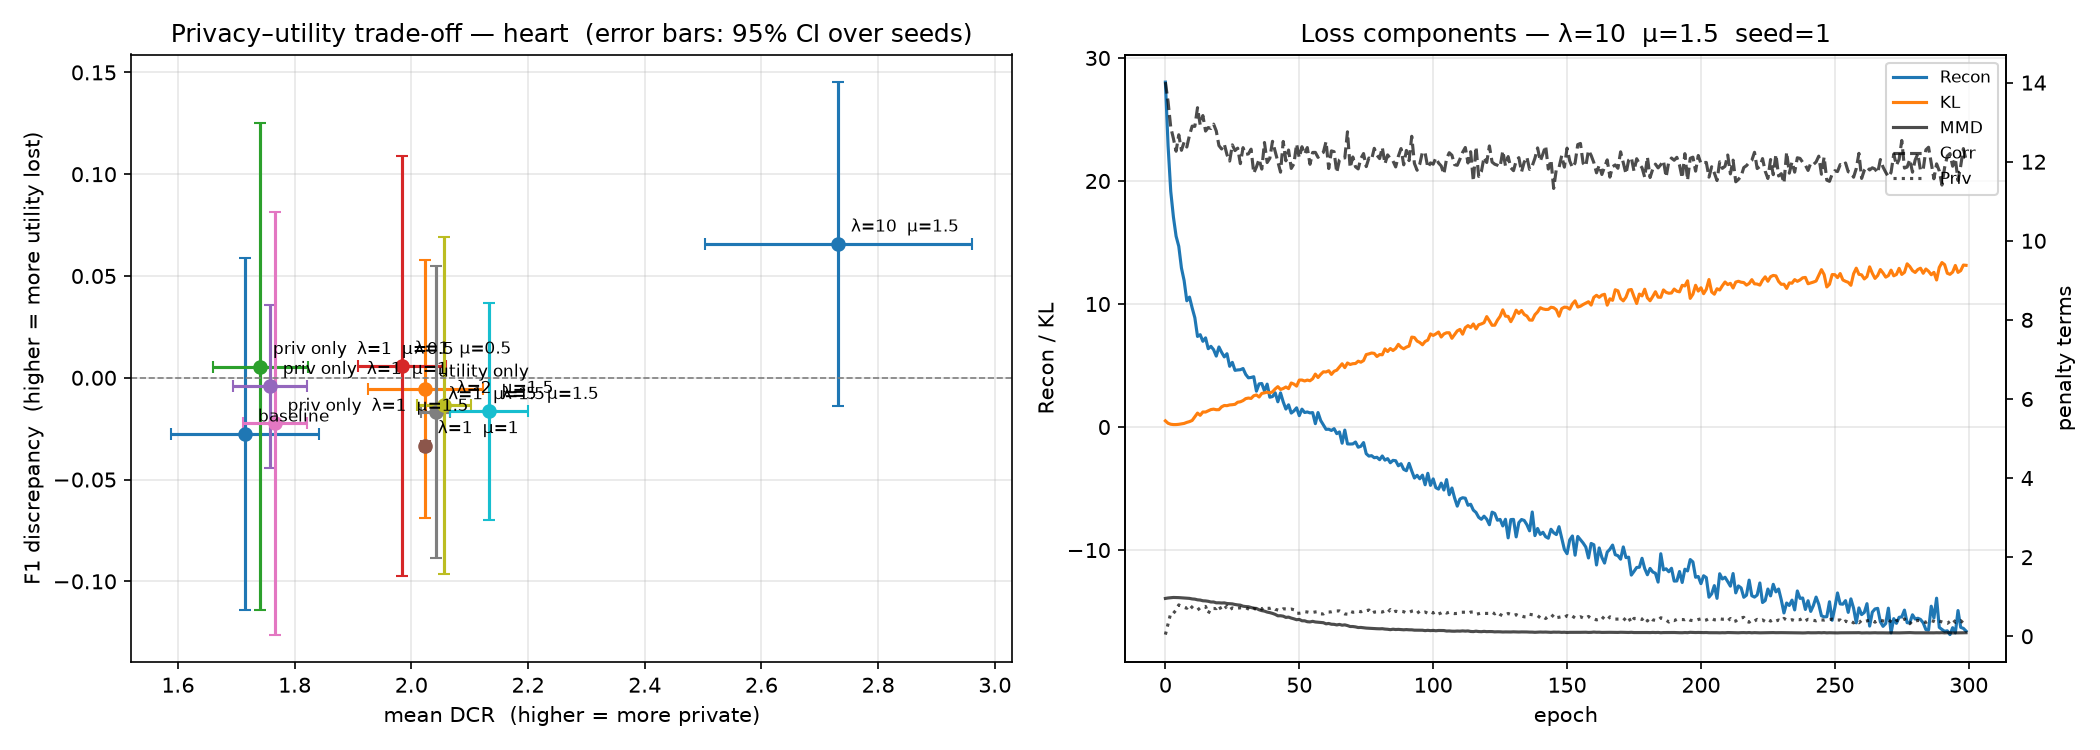
\includegraphics[width=\textwidth]{tradeoff_heart_batch_size32_epochs300.png}
\caption{Left: F1 discrepancy against mean DCR on Heart Disease, one point per
configuration, error bars are 95\% confidence intervals over seeds, collapse
regime excluded. Right: loss components over training for one $\lpriv = 10$,
$\mu = 1.5$ run.}
\label{fig:heart}
\end{figure}

Table~\ref{tab:heart-sweep} shows three regimes.

\paragraph{Regime I, free lunch ($\lpriv \le 5$).}
Privacy improves and nothing is paid for it. F1 discrepancy is
indistinguishable from zero and the distributional metrics move by a few
percent, within their intervals. The DCR gain over baseline is resolved
already at $\lpriv = 1$ ($2.04 \pm 0.03$ against $1.72 \pm 0.13$).

\paragraph{Regime II, trade-off ($\lpriv = 10$, $\mu = 1.5$).}
Mean DCR increases by 33\% ($2.73 \pm 0.23$, clearly separated from
$\lpriv = 5$), the worst-case tail by 47\%, and disclosure is zero. A cost
appears at the same time, but with five seeds only part of it is resolved.
Mean EMD rises to $2.46 \pm 0.62$ against a baseline of $1.36 \pm 0.44$, which
is a real difference. F1 discrepancy is $0.07 \pm 0.08$, an interval that
includes zero, so the downstream-utility cost is an estimate we cannot
distinguish from no cost. Correlation distance ($2.28 \pm 0.32$) is not
separated from the baseline either. This is the operating point where privacy
starts to have a price, and the price is visible in the marginals
(\S\ref{sec:results:features}) more clearly than in F1.

\paragraph{Regime III, collapse ($\mu = 2$ or $\lpriv = 50$).}
\label{sec:results:collapse}
Mean DCR saturates around 6.3 regardless of the exact settings, EMD grows by a
factor of about twenty, and in one run synthetic F1 is exactly equal to the
majority-class baseline, meaning the generated target column collapsed to a
single value. The confidence intervals in these rows are very wide
($23.6 \pm 21.2$ for EMD, $0.22 \pm 0.57$ for F1 discrepancy); the runs
disagree with each other about \emph{how} the collapse happens, which is
itself a sign that the generator has left the data manifold. Privacy is
``perfect'' because the samples do not resemble anyone.

Two methodological findings come out of Regime III. The first is that
\emph{fixed-bandwidth MMD saturates}: it moved from 0.018 to 0.032 while EMD
moved from 1 to 25. Once the two distributions stop overlapping, every
cross-kernel term is close to zero and MMD$^2$ flattens to a constant. As an
evaluation metric it under-reports gross failure; as a loss term its gradient
vanishes exactly when it is needed most, which is why it could not restrain
the hinge at $\lpriv = 50$. The second is that \emph{NNDR inverts off the
manifold}: it rose to 0.95 in the collapse regime, which the usual reading
would interpret as excellent generalization. That reading is wrong here,
because a row that is far from all real records has equidistant neighbours for
trivial reasons. NNDR is only interpretable together with DCR.

A third observation concerns the measurement itself. The 95\% interval for F1
discrepancy is about $\pm 0.08$ at \emph{every} $\lpriv$ in
Table~\ref{tab:heart-sweep}, including where the mean is zero. This is the
resolution limit of a 60-row test split, not a property of the generator, and
it is why the $\lpriv = 10$ cost cannot be separated from zero. The
distributional metrics do not have this limit and show the cost. On small
datasets, distributional metrics can resolve the trade-off while downstream
predictive metrics cannot.

\subsection{Adult: the same penalty appears to be free}
\label{sec:results:adult}

\begin{table}[htbp]
\caption{UCI Adult, 3 seeds. $\pm$ is the 95\% CI half-width.}
\label{tab:adult}
\centering\small
\begin{adjustbox}{max width=\textwidth}
\begin{tabular}{@{}lrrrrrr@{}}
\toprule
configuration & F1 disc & MMD & corr.\ dist & DCR mean & DCR 5th & disclosure \\
\midrule
baseline      & $0.042 \pm 0.031$ & 0.0035 & $0.87 \pm 0.22$ & $1.11 \pm 0.07$ & $0.31 \pm 0.07$ & 13.4\% \\
utility only  & $0.048 \pm 0.004$ & 0.0021 & $0.69 \pm 0.09$ & $1.36 \pm 0.19$ & $0.41 \pm 0.05$ & 8.5\% \\
both ($\lpriv=10$, $\mu=1.5$) & $\mathbf{0.036 \pm 0.005}$ & 0.0022 & $0.73 \pm 0.18$ & $\mathbf{2.37 \pm 0.23}$ & $\mathbf{0.78 \pm 0.11}$ & $\mathbf{1.8\%}$ \\
\bottomrule
\end{tabular}
\end{adjustbox}
\end{table}

\begin{figure}[htbp]
\centering
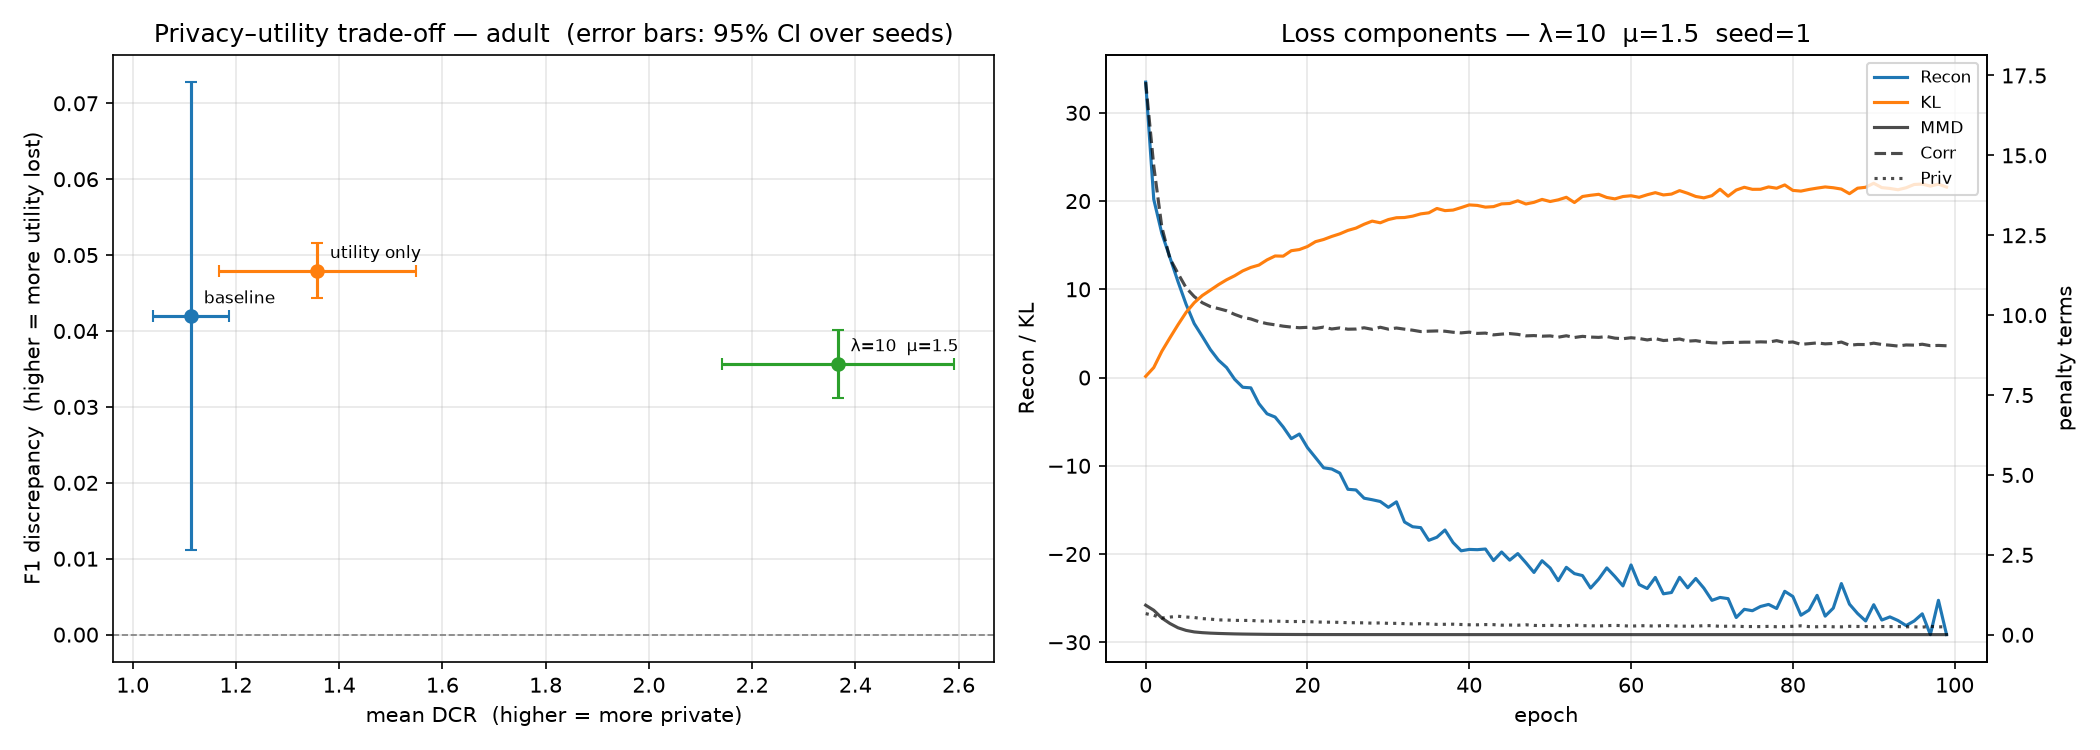
\includegraphics[width=\textwidth]{tradeoff_adult_batch_size500.png}
\caption{Adult: trade-off (left, error bars are 95\% CIs) and loss
components (right). Note that $\Lpriv$ plateaus at a non-zero value instead of
decaying: the model carries a constant cost without visible strain.}
\label{fig:adult}
\end{figure}

On Adult, the configuration that was the knee of the Heart curve improves
everything at once by the aggregate metrics (Table~\ref{tab:adult}). Mean DCR
more than doubles ($2.37 \pm 0.23$ against $1.11 \pm 0.07$), the
5th-percentile DCR grows by a factor of 2.5, disclosure drops from 13\% to
2\%, and F1 discrepancy does not get worse: $0.036 \pm 0.005$ against a
baseline of $0.042 \pm 0.031$. The two intervals overlap, so we cannot claim
an improvement over the baseline, but the loss-aware value is clearly below
the utility-only one ($0.048 \pm 0.004$). MMD and correlation distance are
both at or better than baseline, the latter within overlapping intervals. F1
is now a much more precise instrument ($\pm 0.005$ against $\pm 0.08$ on
Heart, since the test split has 9{,}600 rows), which confirms the
resolution-limit explanation by contrast; the baseline's wider interval
($\pm 0.031$) comes from one seed and is the exception.

The utility-only row is interesting for a different reason. It improved MMD by
40\% and correlation distance by 20\% while F1 discrepancy moved slightly in
the wrong direction. The F1 intervals overlap with the baseline, so we do not
consider this firm, but it is the second time two ``utility'' metrics point in
different directions: matching moments does not guarantee that the decision
boundary a classifier needs is preserved. We read this as an argument against
reporting a single utility number.

\subsection{Diabetes: density is not row count}
\label{sec:results:diabetes}

\begin{table}[htbp]
\caption{Diabetes 130-US Hospitals, 3 seeds per row; $\mu = 1.5$ and
$\lmmd = 1$, $\lcorr = 0.5$ wherever $\lpriv > 0$. $\pm$ is the 95\% CI
half-width.}
\label{tab:diabetes}
\centering\small
\begin{adjustbox}{max width=\textwidth}
\begin{tabular}{@{}lrrrrrrr@{}}
\toprule
$\lpriv$ & F1 disc & F1 synth & MMD & mean EMD & corr.\ dist & DCR mean & DCR 5th \\
\midrule
0 (baseline)     & $0.004 \pm 0.001$ & 0.838 & 0.0019 & $3.85 \pm 0.44$ & $4.37 \pm 0.43$ & $2.48 \pm 0.05$ & $1.48 \pm 0.05$ \\
0 (utility only) & $0.004 \pm 0.001$ & 0.838 & 0.0015 & $2.23 \pm 3.16$ & $2.76 \pm 0.45$ & $3.13 \pm 0.10$ & $1.79 \pm 0.13$ \\
2  & $0.004 \pm 0.002$ & 0.838 & 0.0015 & $\mathbf{1.66 \pm 1.67}$ & $\mathbf{2.65 \pm 0.45}$ & $3.35 \pm 0.10$ & $1.98 \pm 0.13$ \\
5  & $0.048 \pm 0.042$ & 0.794 & 0.0015 & $3.52 \pm 1.16$ & $3.29 \pm 0.52$ & $7.32 \pm 1.25$  & $3.86 \pm 0.36$ \\
10 & $0.069 \pm 0.203$ & 0.773 & 0.0016 & $5.58 \pm 2.71$ & $3.05 \pm 0.44$ & $10.6 \pm 8.2$  & $9.13 \pm 9.43$ \\
\bottomrule
\end{tabular}
\end{adjustbox}
\end{table}

\begin{figure}[htbp]
\centering
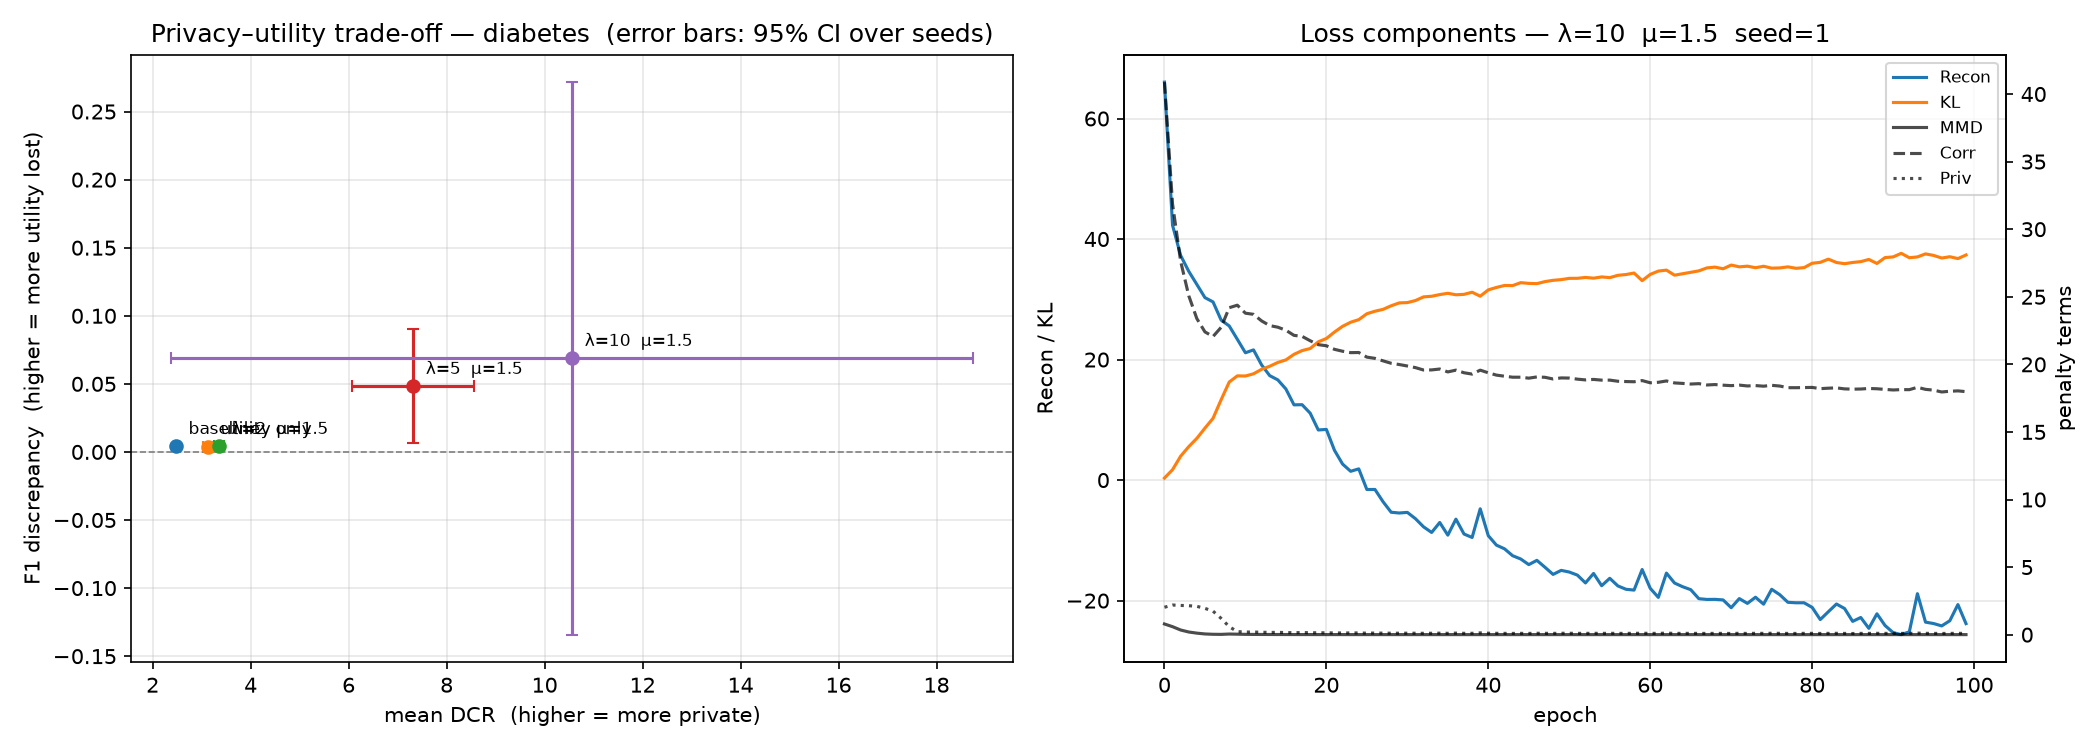
\includegraphics[width=\textwidth]{tradeoff_diabetes_batch_size500.png}
\caption{Diabetes: trade-off (left, error bars are 95\% CIs) and loss
components for a $\lpriv = 5$ run (right). Note the discontinuity in DCR
between $\lpriv = 2$ and $5$: the transition to the collapse regime is a jump
rather than a slope.}
\label{fig:diabetes}
\end{figure}

Diabetes has twice as many rows as Adult and still pays for privacy
(Table~\ref{tab:diabetes}, Figure~\ref{fig:diabetes}). The knee is between
$\lpriv = 2$ and $5$, earlier than on Heart, and it is sharp: mean DCR more
than doubles in that single step ($3.35 \pm 0.10 \to 7.32 \pm 1.25$), while
the same interval on Heart moved it from $2.06$ to $2.13$. The generator seems
to stay on the manifold until it cannot, and then leaves it. NNDR jumping from
$0.91$ to $0.96$ at the same point is the off-manifold signature discussed in
\S\ref{sec:results:collapse}. At $\lpriv = 10$ the interval on mean DCR is
$\pm 8.2$: one seed reached $14.3$, the other two about $8.7$. That spread is
itself a symptom of collapse, and we treat $\lpriv = 5$ rather than $10$ as
the reliable description of what happens past the knee. Below the knee,
$\lpriv = 2$ is the best configuration in the table: lowest EMD and
correlation distance of any row (the correlation improvement over baseline,
$2.65 \pm 0.45$ against $4.37 \pm 0.43$, is well resolved; the EMD one is
not), DCR $+35\%$ over baseline, F1 unchanged.

Two more points. First, F1 discrepancy is degenerate on this dataset for a
third, different reason: the target is roughly $89/11$ imbalanced and weighted
F1 sits on a ceiling where the synthetic-trained classifier predicts the
majority class ($F1_{\text{synth}} = 0.838 = $ majority baseline below the
knee) and the real-trained one barely does better ($0.842$). Above the knee
$F1_{\text{synth}}$ drops \emph{below} the majority baseline, which means the
synthetic label marginal itself has been distorted. Here F1 discrepancy
measures corruption of the target distribution rather than loss of predictive
signal, and at $\lpriv = 5$ its interval ($0.048 \pm 0.042$) only just
excludes zero. Heart's F1 was limited by noise, Adult's was informative, and
Diabetes's is limited by class imbalance; positive-class F1 or AUROC would
have been a better choice. Second, the utility terms improved privacy again
(DCR $3.13 \pm 0.10$ against $2.48 \pm 0.05$), together with a resolved 37\%
reduction in correlation distance. Across three datasets spanning two orders
of magnitude in size, the direction is the same and the DCR difference is
resolved on all three.

\subsection{Where the cost lands: per-feature analysis}
\label{sec:results:features}

Every run stores the EMD of each column separately. Averaging across seeds and
comparing each $\lpriv$ with the plain baseline tells us \emph{which} columns
pay for privacy. For a binary label-encoded column, EMD equals the absolute
shift in proportion, so those entries can be read directly as percentage
points. Figure~\ref{fig:features} shows the heatmaps for Heart and Adult,
Figure~\ref{fig:features-diabetes} the one for Diabetes, and
Table~\ref{tab:features} lists the columns that moved most.

\begin{table}[htbp]
\caption{Per-feature EMD, mean over seeds. $k$ = number of distinct values.
For binary columns EMD is the absolute difference in proportion. Adult rows
are the top of the ranking by standardized change (EMD change divided by the
real column's standard deviation); the full ranking's top six are
native-country, race, workclass, sex, income, relationship, all categorical,
four of them protected or sensitive attributes and one the target.}
\label{tab:features}
\centering\small
\begin{tabularx}{\textwidth}{@{}l l l r r Y@{}}
\toprule
dataset & config & column & baseline & EMD & reading (deviation from real; baseline in parentheses) \\
\midrule
Adult & $\lpriv=10$ & native-country ($k$=42) & 1.4 & 9.1 & $+1.0$ sd; largest standardized shift \\
Adult & $\lpriv=10$ & race ($k$=5) & 0.16 & 0.91 & $+0.9$ sd \\
Adult & $\lpriv=10$ & sex ($k$=2) & 0.010 & 0.144 & sex ratio off by 14 pp (1 pp) \\
Adult & $\lpriv=10$ & income ($k$=2, target) & 0.013 & 0.111 & positive rate off by 11 pp (1 pp) \\
Adult & $\lpriv=10$ & fnlwgt, education, hours/wk & --- & --- & \emph{improved} ($\times 0.3$--$0.6$) \\
\midrule
Heart & $\lpriv=10$ & num ($k$=2, target) & 0.013 & 0.229 & disease prevalence off by 23 pp (1 pp) \\
Heart & $\lpriv=10$ & sex ($k$=2) & 0.057 & 0.118 & sex ratio off by 12 pp (6 pp) \\
Heart & $\lpriv=50$ & chol & 6.3 & 280 & mean cholesterol off by 280 mg/dL \\
Heart & $\lpriv=50$ & trestbps & 5.3 & 59 & resting BP off by 59 mmHg \\
Heart & $\lpriv=50$ & thalach & 3.7 & 62 & max heart rate off by 62 bpm \\
Heart & $\lpriv=50$ & age & 2.0 & 20.6 & age off by 20 years \\
\midrule
Diabetes & $\lpriv=2$ & diag\_1 ($k$=656) & 46.5 & 8.5 & \emph{improved} $5\times$ \\
Diabetes & $\lpriv=2$ & gender ($k$=2) & 0.125 & 0.012 & \emph{improved} $10\times$ \\
Diabetes & $\lpriv=10$ & readmitted ($k$=2, target) & 0.11 & 0.75 & readmission rate off by 75 pp (11 pp) \\
Diabetes & $\lpriv=10$ & diabetesMed ($k$=2) & 0.016 & 0.39 & medication flag off by 39 pp (2 pp) \\
Diabetes & $\lpriv=10$ & acarbose ($k$=4) & 0.003 & 0.33 & rare drug ($\sim$0.3\% real) in $\sim$1/3 of rows \\
\bottomrule
\end{tabularx}
\end{table}

\begin{figure}[htbp]
\centering
\begin{subfigure}[t]{0.49\textwidth}
  \centering
  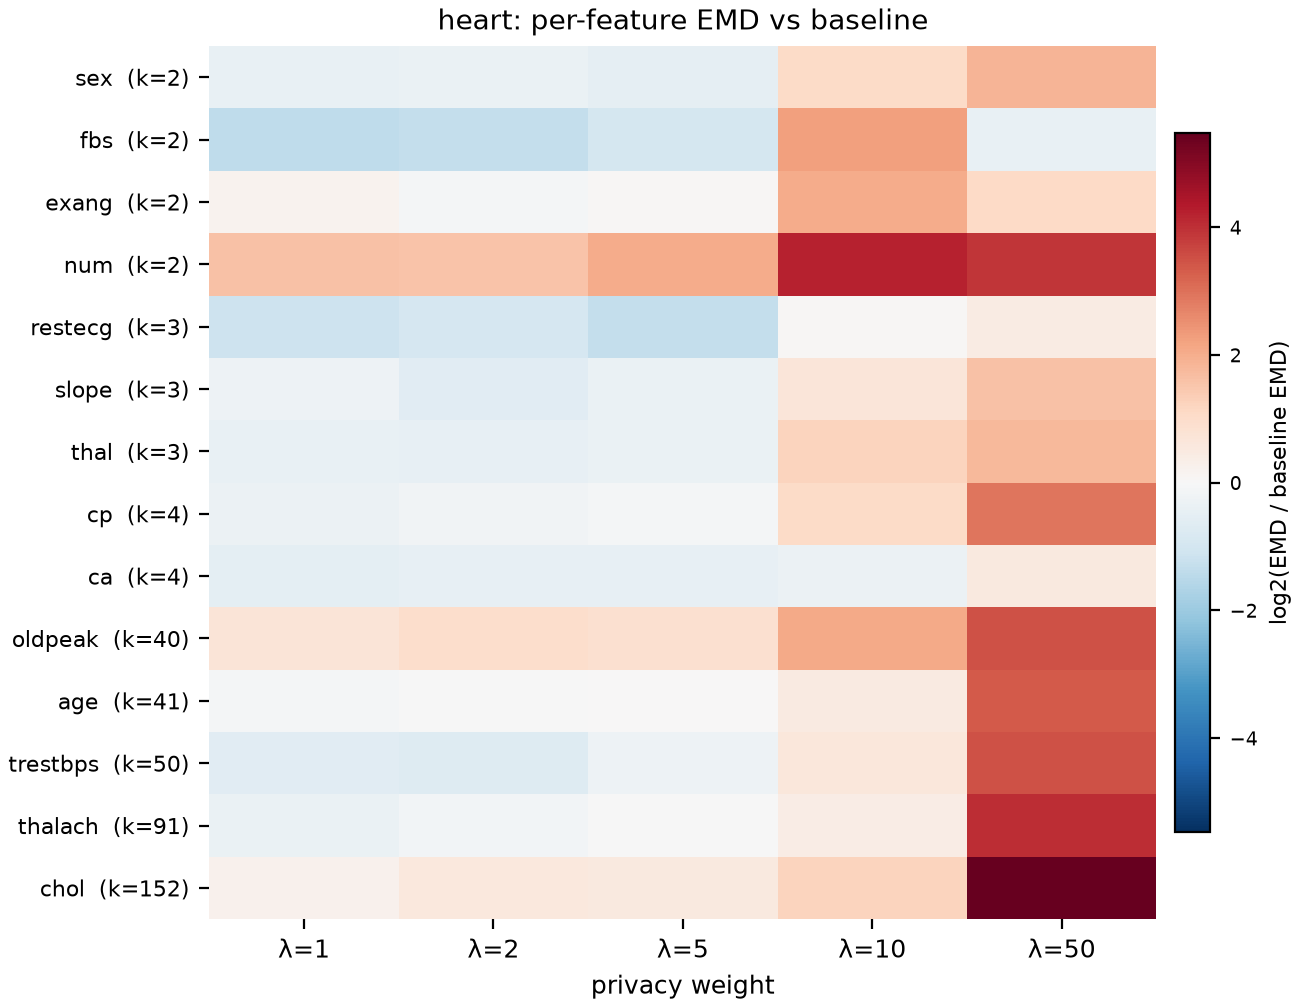
\includegraphics[width=\linewidth]{feature_emd_heart_batch_size32_epochs300.png}
  \caption{Heart Disease}
\end{subfigure}\hfill
\begin{subfigure}[t]{0.49\textwidth}
  \centering
  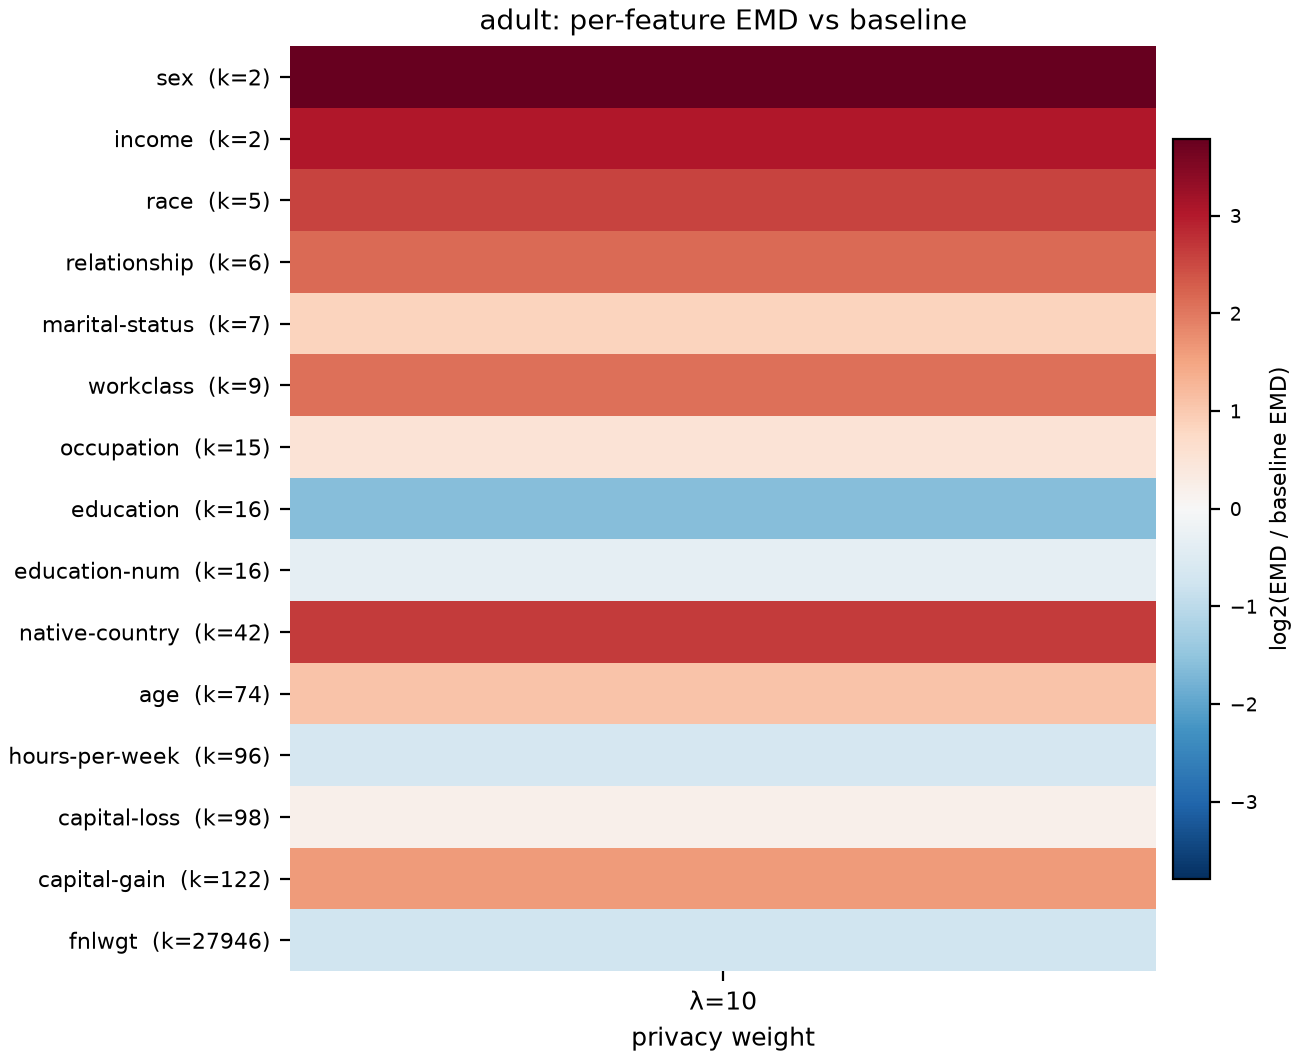
\includegraphics[width=\linewidth]{feature_emd_adult_batch_size500.png}
  \caption{UCI Adult}
\end{subfigure}
\caption{Per-feature EMD relative to the plain baseline, $\log_2$ ratio:
red = worse than baseline, blue = better. Rows sorted by cardinality $k$
(in parentheses); columns are $\lpriv$. On Heart the continuous clinical
measurements dominate the collapse column; on Adult the categorical and
sensitive columns turn red while the continuous ones turn blue.}
\label{fig:features}
\end{figure}

\begin{figure}[p]
\centering
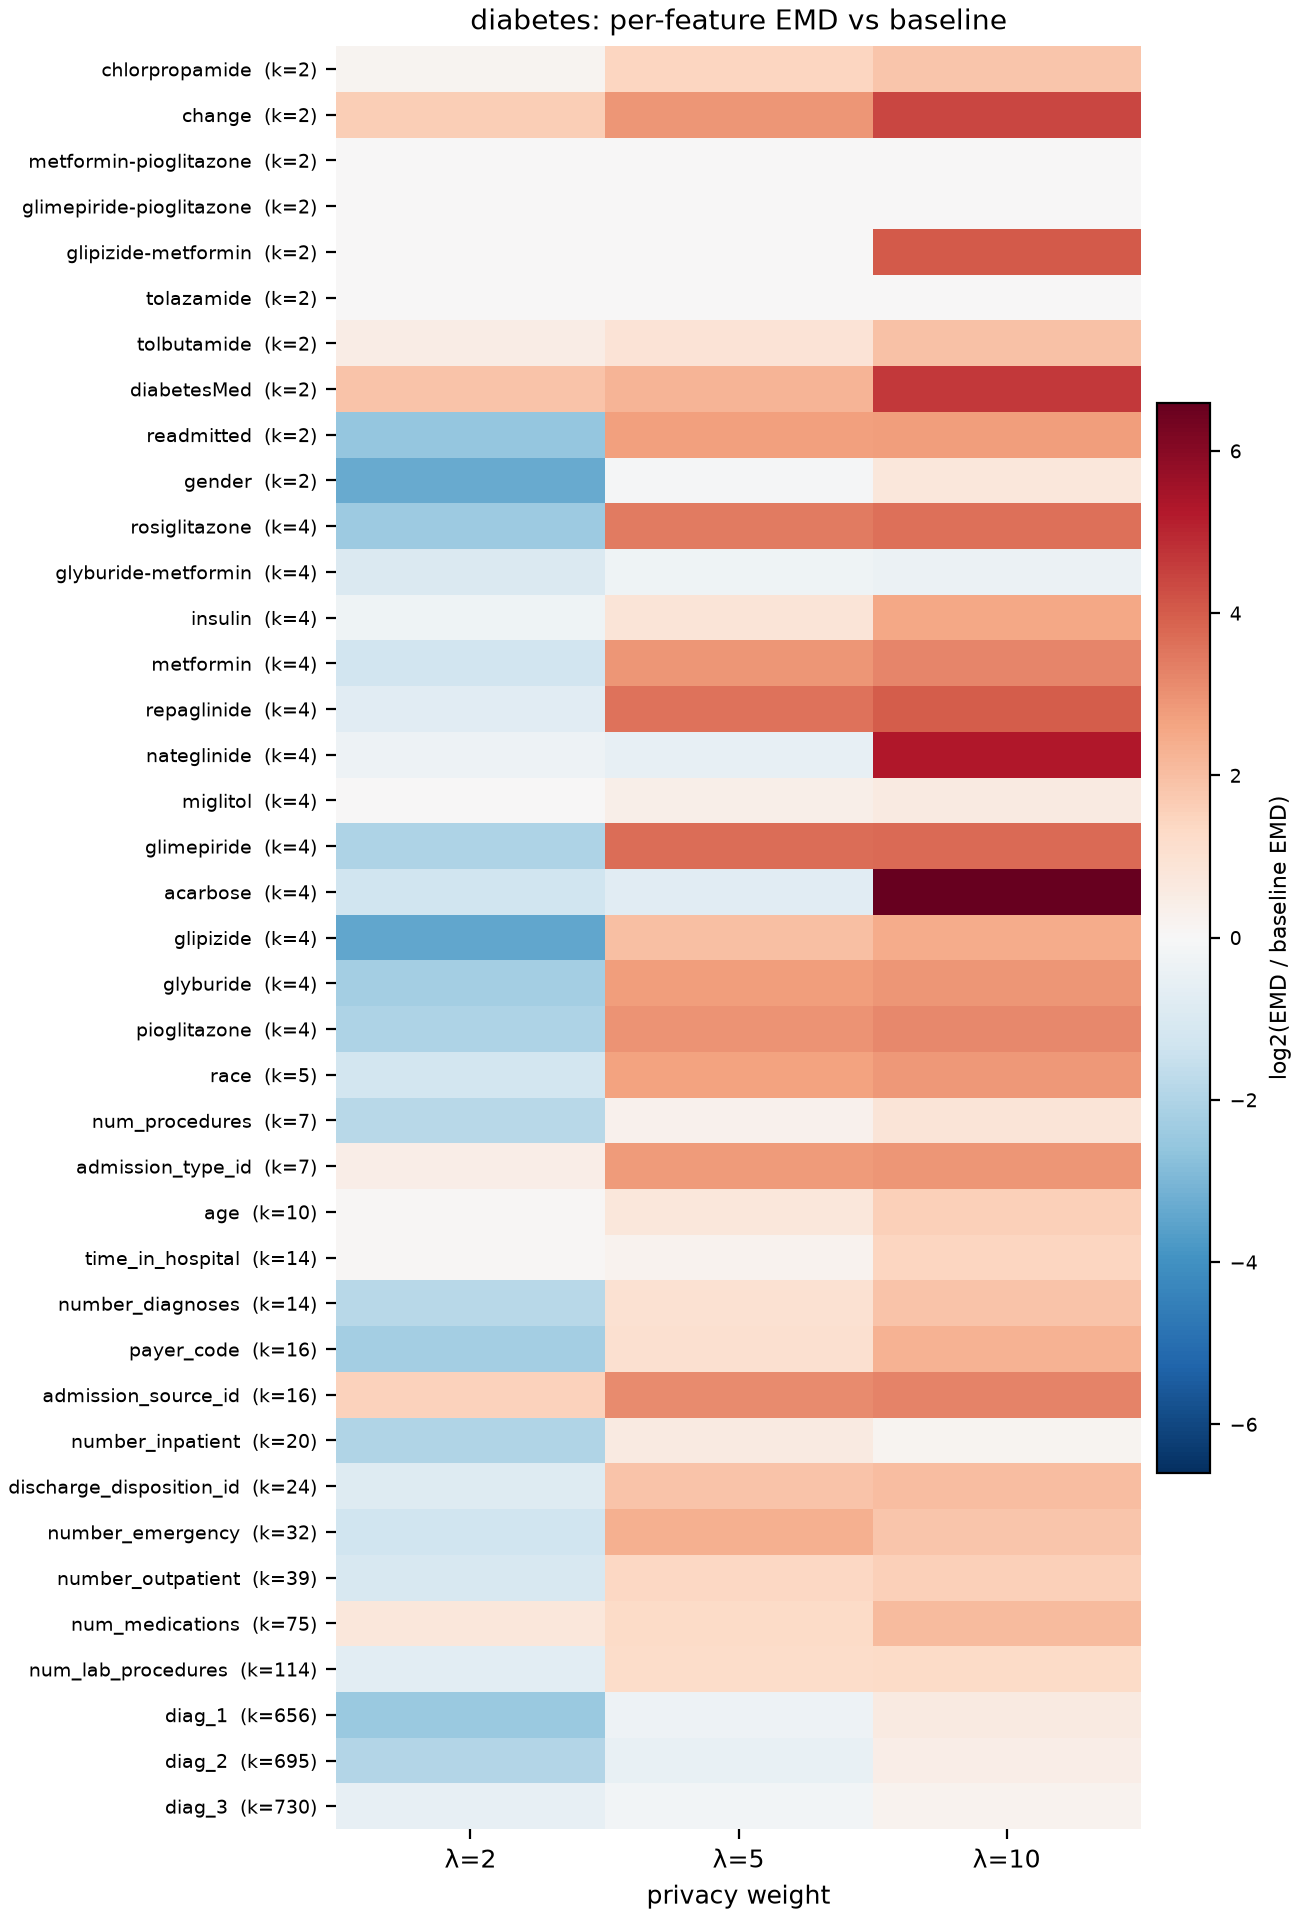
\includegraphics[height=0.88\textheight,keepaspectratio]{feature_emd_diabetes_batch_size500.png}
\caption{Diabetes 130-US Hospitals: per-feature EMD relative to baseline,
same encoding as Figure~\ref{fig:features}; constant columns omitted. The
$\lpriv = 2$ column is almost entirely blue; the $\lpriv \ge 5$ columns are
dominated by the binary medication flags and the readmission target.}
\label{fig:features-diabetes}
\end{figure}

\paragraph{The Adult ``free lunch'' was not free.}
This is the most important block of Table~\ref{tab:features}. At
$\lpriv = 10$ on Adult every aggregate metric improved
(Table~\ref{tab:adult}), and we called it the free-lunch region. If we rank
the columns by standardized change, the six that moved most are
native-country, race, workclass, sex, income and relationship. All of them are
categorical, four are protected or sensitive attributes and one is the target,
while the continuous columns are at the bottom of the ranking or actually
\emph{improved}. The sex ratio ended up 14 points away from the real one and
the income rate 11 points. The cost fell exactly on the columns a fairness
audit would look at first, and no aggregate metric registered it. Weighted F1
is scored on real test rows, and a classifier trained on a table with too many
rows of one sex still classifies real rows well. Pearson correlation is
almost invariant to a marginal shift. A fixed-bandwidth MMD in fourteen
dimensions hardly registers a single binary coordinate moving. In other words,
the verdict ``free'' came from instruments that are structurally unable to see
the ethically relevant distortion. \S\ref{sec:results:adult} is correct for
the metrics it reports; we withdraw its interpretation.

\paragraph{What breaks is the sparsest region of each column.}
Our cardinality test gave inconsistent results across datasets ($r = +0.76$
on Heart, $-0.56$ on Adult, undefined on Diabetes), and we think this is
because cardinality is the wrong variable. What degrades is the minority value
of binary columns (sex, the target), rare categories (acarbose, prescribed to
0.3\% of real patients and present in a third of synthetic rows), and the
tails of continuous columns (cholesterol off by 280~mg/dL in the collapse
regime). High-cardinality columns sometimes \emph{improve}. The hinge appears
to escape real records by moving probability mass into whatever region of each
column is least populated. This is the density account of
\S\ref{sec:results:diabetes} at the level of individual features, and it also
suggests a mechanism. It also means that the collapse regime does not just
produce implausible records; it produces records that systematically
over-represent rare categories and minority classes.

\paragraph{Regime II costs are target-rate shifts.}
On Heart at $\lpriv = 10$ the ``$0.07$ of F1'' we reported in
\S\ref{sec:results:heart-curve} corresponds to a 23-point shift in disease
prevalence. On Diabetes at $\lpriv \ge 5$ the target shifts by up to 75
points, which inverts the synthetic majority class and explains why synthetic
F1 fell below the majority baseline. On every dataset, the knee of the
trade-off is the point where the generator starts to misrepresent how common
the outcome is.

\paragraph{Low $\lpriv$ is a real sweet spot.}
At $\lpriv = 2$ on Diabetes almost every column improves, the 656-value
diagnosis code by a factor of five and gender by a factor of ten. At
$\lpriv \le 5$ on Heart most ratios are below one. The free-lunch region of
\S\ref{sec:results:heart-curve} exists, but it is narrower than the aggregate
metrics suggested, and on Adult it does not extend to $\lpriv = 10$.

\subsection{Synthesis}

\begin{table}[htbp]
\caption{The three datasets on one axis, ordered by where the trade-off
begins.}
\label{tab:synthesis}
\centering\small
\begin{tabularx}{\textwidth}{@{}l r r l Y r@{}}
\toprule
dataset & rows & columns & density & privacy penalty at $\lpriv = 10$ & knee ($\lpriv$) \\
\midrule
Adult    & 37{,}000 & 14        & dense              & aggregate metrics: free; protected-attribute marginals: 14 pp sex shift & $> 10$ (aggr.) \\
Heart    & 237    & 13          & sparse (few rows)  & costs utility & 5--10 \\
Diabetes & 57{,}000 & $\approx 40$ & sparse (many dims) & costs utility & 2--5 \\
\bottomrule
\end{tabularx}
\end{table}

Table~\ref{tab:synthesis} summarizes the central empirical claim of the
project. The hinge pushes each generated row away from its nearest real row.
On a dense manifold the row ends up next to another plausible but fictional
record and the distribution is preserved. On a sparse one the nearest empty
space is off the manifold, the row becomes an implausible record and the
distribution degrades. A dataset can be sparse because it has few rows (Heart)
or because it has many dimensions (Diabetes: volume grows exponentially with
dimensionality, and 57{,}000 rows in forty dimensions are much thinner than
37{,}000 in fourteen). What sets the price of a privacy penalty seems to be
how densely the records fill the space the generator works in, rather than the
number of records. The ordering of the knees is consistent with this account.
It is also consistent with the hinge-scale confound discussed in
\S\ref{sec:limitations}, and we are not able to separate the two with our
runs.

% =============================================================================
\section{Discussion}
\label{sec:discussion}

\paragraph{Privacy versus utility is an incomplete framing.}
Regime I shows that on every dataset a term designed only to improve
distributional fidelity also improved every privacy indicator, by 17 to 26\%
in mean DCR. Regularizing towards population-level statistics spreads
generated samples across the distribution instead of clustering them on
training records, and better generalization turns out to be better privacy.
The common picture of two quantities on opposite ends of a dial misses this.
There is a region in which both improve, and a practitioner who does not look
for it will not find it. The per-feature analysis makes this region narrower
(on Adult it does not reach $\lpriv = 10$) but does not remove it: at
$\lpriv = 2$ on Diabetes the diagnosis codes, the gender marginal and the
privacy indicators all improved together.

\paragraph{Aggregate utility metrics are blind to the distortions that matter
most.}
The clearest result of this study is a negative one. Every aggregate utility
metric we used (MMD, correlation distance, downstream F1) reported the Adult
$\lpriv = 10$ configuration as an improvement, while the sex ratio moved by 14
points and the income rate by 11. These are the columns a fairness audit would
check first, and the standard utility toolkit could not see them move. A
synthetic dataset can pass every fidelity check in the literature and still
misrepresent who is in it. Per-column marginal checks on protected attributes
and on the target are therefore not optional additions to a utility
evaluation. Without them, the evaluation does not measure what it claims to
measure.

\paragraph{A privacy score without a utility floor is meaningless.}
Regime III shows that every privacy indicator we use can be trivially
maximized by a generator that produces noise. This is obvious once stated but
is routinely ignored in practice: ``our synthetic data has DCR of $x$'' is not
a statement about privacy unless it comes with a statement about what the data
is still good for. Any evaluation protocol, and any regulation, that scores
privacy without also scoring utility can be gamed by destroying the data.

\paragraph{The trade-off is a decision, and this is where it lives.}
Regime II is the region where privacy has a price, and the price is now a
number with an uncertainty attached. On Heart Disease, a 33\% increase in the
distance between synthetic and real patients was bought with a downstream F1
cost of $0.07 \pm 0.08$, an interval that includes zero, and with a
measurably distorted marginal distribution. A data-protection officer, a
clinical researcher and a patient representative would weigh that offer
differently, and one of the things they would have to weigh is how uncertain
the cost is. The contribution of the loss-aware formulation is not that it
resolves the disagreement, but that it produces a concrete offer for them to
disagree about: four numbers, $\lmmd, \lcorr, \lpriv, \mu$, that can be
documented, argued over and set by whoever has the standing to set them. A
stock generator embeds the same decision in defaults that no stakeholder ever
sees.

\paragraph{The price falls on those who can least afford it.}
Table~\ref{tab:synthesis} has an ethical reading that we did not anticipate,
and that we consider the most important point of this report. The same
penalty was free on a dense census dataset, at least by the aggregate metrics,
and costly on both sparse ones. Sparsity comes from having few records or from
describing each record richly. Small populations, rare conditions, detailed
clinical histories and under-represented groups are exactly the settings in
which a privacy failure does the most harm, and they are also the settings in
which protection is most expensive in terms of utility. The per-feature
analysis sharpens this to the level of single attributes. The hinge protects
individuals by moving generated mass into the least populated regions of every
column, which means it systematically inflates minority classes and rare
categories. A synthetic table made private in this way over-represents the
very groups whose sparsity made them vulnerable in the first place, and it
misstates how common the outcome is. Any policy that fixes a single
privacy-utility weighting for all datasets will therefore either under-protect
the sparse population or over-pay on the dense one, and where a payment is
made, it is made in the demographic marginals. The weighting has to be set per
dataset, the density of the data is one of the things whoever sets it needs to
see, and the check on what was paid has to be done column by column.

\paragraph{Against the baselines.}
Table~\ref{tab:baselines} lets us position the loss-aware model. On Adult at
$\lpriv = 10$ it has F1 discrepancy $0.036 \pm 0.005$, against $0.053$,
$0.058$ and $0.145$ for CTGAN, TVAE and the copula, and mean DCR
$2.37 \pm 0.23$ against $1.68$, $1.18$ and $3.08$. It is therefore at least as
useful as every baseline (the CTGAN interval, $\pm 0.028$ over three seeds,
overlaps it) and clearly more private than both neural ones. On Heart at the
$\lpriv \le 5$ sweet spot it matches the copula's privacy with somewhat better
correlation preservation. On Diabetes at $\lpriv = 2$ the copula is still
more private and the two are close on fidelity. A trained penalty does not
make the simple statistical model obsolete, but it does make the neural one
competitive with it on privacy while keeping the neural one's utility.

\paragraph{Metrics disagree, and that is useful information.}
Four times in this study one metric moved while another did not: MMD saturated
while EMD exploded; NNDR rose while DCR indicated the samples had left the
manifold; MMD and correlation improved while F1 drifted; and every aggregate
utility metric improved while the sex and income marginals shifted by more
than ten points. Each of these disagreements pointed to a real property of the
data or of the metric. A single utility number and a single privacy number
would have hidden all four.

% =============================================================================
\section{Limitations}
\label{sec:limitations}

\begin{itemize}[nosep]
  \item \textbf{Few seeds.} Most configurations have three seeds, the Heart
        transition region five. The 95\% intervals are wide as a result, and
        several of the utility-cost differences we describe are not
        statistically resolved: the Heart $\lpriv = 10$ F1 cost includes zero,
        the Adult loss-aware F1 improvement over baseline is not separated,
        and the Diabetes $\lpriv = 10$ DCR has an interval of $\pm 8$. The
        privacy differences (DCR, disclosure) are resolved throughout, and the
        marginal shifts in \S\ref{sec:results:features} are large relative to
        their baselines, so the main claims stand; the finer utility
        comparisons would need more seeds.
  \item \textbf{No formal guarantee.} Our privacy indicators simulate specific
        attacks and measure their empirical success. They are not
        differential-privacy bounds, they do not compose, and they would not
        detect an attack we did not model \citep{stadler2022groundhog}.
  \item \textbf{Inference risk equals downstream utility.} Because the
        sensitive column and the prediction target coincide in all three
        datasets, the inference-risk metric is numerically identical to
        $F1_{\text{synth}}$. It is not an independent privacy signal here. A
        separate sensitive attribute (for example race or sex) would make it
        one, and would raise the group-fairness questions we did not address.
  \item \textbf{Fixed-bandwidth MMD.} It saturates once the distributions
        separate, both as a metric and as a loss term. A multi-scale kernel
        would reduce this problem.
  \item \textbf{Absolute thresholds.} The disclosure-rate threshold ($0.5$)
        and the evaluation-time DCR are expressed in standardized raw-feature
        units, which grow with dimensionality, so absolute values are not
        comparable across datasets (baseline disclosure is 13\% on Adult and
        0\% on Diabetes for this reason). The training margin was made relative
        (\S\ref{sec:fixes}); the evaluation thresholds should be as well.
  \item \textbf{Hinge magnitude scales with dimension.} The margin $m$ is
        relative but the penalty $\max(0, m - d_i)$ is not, so a fixed
        $\lpriv$ is effectively stronger in a wider transformed space. The
        ordering of the knees in Table~\ref{tab:synthesis} is predicted by
        this confound as well as by the density account, so the two cannot be
        separated with our runs. Normalizing the hinge to
        $\max(0, 1 - d_i/m)$ is a one-line fix that would require re-running
        everything.
  \item \textbf{F1 discrepancy is fragile.} It is limited by noise on Heart
        (60-row test set) and by class imbalance on Diabetes (weighted F1 on
        an 89/11 target). Only on Adult was it a usable instrument.
        Positive-class F1 or AUROC should replace weighted F1.
  \item \textbf{Mean EMD is in raw units} and is dominated by high-range
        columns; a per-feature standardized version would allow cross-dataset
        comparison.
  \item \textbf{Fairness was out of scope, and the results show it should
        not have been.} The utility penalties reward faithful reproduction of
        the training distribution, including whatever bias it encodes, and we
        measured neither demographic parity nor equalized odds. The
        per-feature analysis (\S\ref{sec:results:features}) then showed the
        privacy penalty shifting the sex, race and target marginals by 10 to
        75 points while every aggregate utility metric improved or stayed
        flat. Marginal checks on protected attributes belong in the evaluation
        framework rather than in future work.
  \item \textbf{Three datasets, one loss-aware generator family.} The density
        claim rests on three points on one axis. The baseline comparison
        covers three families, but the penalties were added only to TVAE,
        which Table~\ref{tab:baselines} shows to be the least private starting
        point. The free-lunch effect should be tested on CTGAN and the copula
        before being called general.
  \item \textbf{Baseline training budgets were library defaults.} CTGAN's
        Heart result is an artefact of \texttt{batch\_size=500} on 237 rows,
        not a property of the architecture. A fair comparison would tune the
        budgets per dataset as we did for the loss-aware runs.
\end{itemize}

% =============================================================================
\section{Conclusion}

We started this project with the goal of building a synthetic-data generator
that minimizes utility loss under an explicit privacy constraint, and with the
argument that writing the constraint into the objective is ethically
preferable to checking it afterwards. We built the generator and we still
hold the argument. The experiments, however, returned something we had not
asked for. The privacy penalty protects individuals by moving generated
records into the least populated regions of every attribute. As a consequence
it inflates minority classes and rare categories and misstates the outcome
rate, and it does so more strongly the sparser the data. Our evaluation
framework, eight metrics that are standard in the literature, reported an
improvement on the dataset where the sex ratio had moved by fourteen points.
That the populations for whom privacy matters most are the ones for whom it is
most expensive, and that the instruments meant to detect the expense cannot
see it, is an uncomfortable pair of results. It is also the kind of result an
ethics-first framing is supposed to bring out. The loss-aware generator does
not make the decision easier. It makes it visible, per dataset, as four
numbers, and it gives whoever sets those numbers the evidence that they must
be checked column by column, because the aggregate metrics will not show what
was paid.

% =============================================================================
\paragraph{Code and data.}
All code, run reports, figures and the extended technical documentation are at
\url{https://github.com/miky-alt/Loss-Aware-Synthetic-Data-Generation}. Every
number in this report can be reproduced from the
run index with \texttt{src/experiments/plot\_tradeoff.py} and
\texttt{src/experiments/plot\_feature\_emd.py}.

\bibliographystyle{plainnat}
\bibliography{references}

% =============================================================================
\clearpage
\appendix

\section{The loss-aware training loop}
\label{app:algorithm}

Algorithm~\ref{alg:lossaware} is the body of \texttt{LossAwareTVAE.fit()}.
Lines 1--3 and the block from line 9 onward are unchanged from
\texttt{ctgan.TVAE}; lines 4--5 and 12--20 are our additions. With
$\lmmd = \lcorr = \lpriv = 0$ the inserted block is skipped entirely.

\begin{algorithm}[htbp]
\caption{Loss-aware TVAE training}
\label{alg:lossaware}
\begin{algorithmic}[1]
\Require training table $D$; discrete columns; weights $\lmmd, \lcorr, \lpriv$; relative margin $\mu$; bandwidth $\gamma$
\State $T \gets \textsc{DataTransformer}(D)$; \; $X \gets T(D)$ \Comment{mode-specific normalization + one-hot}
\State initialise encoder $E_\phi$, decoder $G_\theta$, optimiser (Adam, weight decay $\ell_2$)
\State $\tilde d_{\text{real}} \gets \operatorname{median}_i \min_{j \ne i} \|X_i - X_j\|_2$ \Comment{on $\le 2000$ rows}
\State $m \gets \mu \cdot \tilde d_{\text{real}}$ \Comment{effective privacy margin}
\For{epoch $= 1 \dots E$}
  \For{each minibatch $x \in X$ of size $B$}
    \State $\mu_z, \sigma_z, \log\sigma_z^2 \gets E_\phi(x)$; \; $z \gets \mu_z + \sigma_z \odot \epsilon$, $\epsilon \sim \mathcal N(0,I)$
    \State $\hat x, \sigma_{\text{dec}} \gets G_\theta(z)$
    \State $\mathcal L \gets \Lrec(\hat x, x, \sigma_{\text{dec}}) + \Lkl(\mu_z, \log\sigma_z^2)$ \Comment{stock TVAE}
    \If{$\lmmd > 0$ or $\lcorr > 0$ or $\lpriv > 0$}
      \State $z' \sim \mathcal N(0, I)^{B}$; \; $r \gets G_\theta(z')$ \Comment{fresh prior batch, not a reconstruction}
      \If{$\lmmd > 0$ or $\lcorr > 0$}
        \State $\tilde x \gets \sigma_{\text{soft}}(r)$ \Comment{$\tanh$ on scalars, softmax on one-hot spans}
        \State $\mathcal L \gets \mathcal L + \lmmd \cdot \textsc{MMD}^2_\gamma(\tilde x, x) + \lcorr \cdot \|\mathrm{Corr}(\tilde x) - \mathrm{Corr}(x)\|_F$
      \EndIf
      \If{$\lpriv > 0$}
        \State $\tilde x^{\text{hard}} \gets \sigma_{\text{hard}}(r)$ \Comment{straight-through one-hot on one-hot spans}
        \State $d_i \gets \min_j \|\tilde x^{\text{hard}}_i - x_j\|_2$ for $i = 1..B$
        \State $\mathcal L \gets \mathcal L + \lpriv \cdot \frac1B \sum_i \max(0, m - d_i)$
      \EndIf
    \EndIf
    \If{$\mathcal L$ is not finite} \textbf{skip step} \EndIf
    \State backpropagate $\mathcal L$; optimiser step; clamp $\sigma_{\text{dec}} \in [0.01, 1]$
    \State log $(\Lrec, \Lkl, \Lmmd, \Lcorr, \Lpriv, \bar d)$
  \EndFor
\EndFor
\end{algorithmic}
\end{algorithm}

Sampling is unchanged from TVAE: draw $z \sim \mathcal N(0,I)$, decode, apply
$\tanh$ and $\arg\max$, and invert the transformer.

% -----------------------------------------------------------------------------
\section{Full per-feature EMD tables}
\label{app:features}

Tables~\ref{tab:feat-heart} and \ref{tab:feat-adult} report every column for
Heart Disease and Adult. The Diabetes table has 45 columns and is provided as
\texttt{experiments/figures/feature\_emd\_diabetes\_batch\_size500.csv}. All
values are mean EMD over seeds, in raw feature units. $k$ is the number of
distinct values in the real column.

\begin{table}[htbp]
\caption{Heart Disease: per-feature EMD by $\lpriv$ ($\mu = 1.5$; baseline
has all $\lambda = 0$). For $k=2$ columns the value is the absolute difference
in proportion.}
\label{tab:feat-heart}
\centering\small
\begin{adjustbox}{max width=\textwidth}
\begin{tabular}{@{}lrrrrrrr@{}}
\toprule
column & $k$ & baseline & $\lpriv{=}1$ & $\lpriv{=}2$ & $\lpriv{=}5$ & $\lpriv{=}10$ & $\lpriv{=}50$ \\
\midrule
sex      & 2   & 0.057 & 0.043 & 0.044 & 0.041 & 0.118 & 0.209 \\
fbs      & 2   & 0.122 & 0.046 & 0.050 & 0.062 & 0.573 & 0.092 \\
exang    & 2   & 0.059 & 0.068 & 0.054 & 0.062 & 0.241 & 0.125 \\
num (target) & 2 & 0.013 & 0.038 & 0.037 & 0.052 & 0.229 & 0.187 \\
restecg  & 3   & 0.264 & 0.119 & 0.141 & 0.107 & 0.278 & 0.362 \\
slope    & 3   & 0.116 & 0.095 & 0.075 & 0.091 & 0.184 & 0.354 \\
thal     & 3   & 0.405 & 0.302 & 0.298 & 0.311 & 0.932 & 1.391 \\
cp       & 4   & 0.197 & 0.157 & 0.171 & 0.181 & 0.402 & 1.505 \\
ca       & 4   & 0.276 & 0.188 & 0.205 & 0.200 & 0.224 & 0.400 \\
oldpeak  & 40  & 0.135 & 0.221 & 0.259 & 0.248 & 0.573 & 1.490 \\
age      & 41  & 2.02  & 1.87  & 2.00  & 2.06  & 2.82  & 20.6 \\
trestbps & 50  & 5.28  & 3.45  & 3.25  & 4.35  & 8.06  & 58.7 \\
thalach  & 91  & 3.70  & 2.87  & 3.30  & 3.63  & 4.96  & 61.7 \\
chol     & 152 & 6.33  & 7.53  & 9.33  & 9.13  & 14.8  & 280.5 \\
\bottomrule
\end{tabular}
\end{adjustbox}
\end{table}

\begin{table}[htbp]
\caption{UCI Adult: per-feature EMD, baseline vs $\lpriv = 10$ ($\mu = 1.5$),
with the ratio and the standardized change used for the ranking in
\S\ref{sec:results:features}. Sorted by standardized change.}
\label{tab:feat-adult}
\centering\small
\begin{adjustbox}{max width=\textwidth}
\begin{tabular}{@{}lrrrrr@{}}
\toprule
column & $k$ & baseline & $\lpriv{=}10$ & ratio & std.\ change \\
\midrule
native-country & 42    & 1.447   & 9.085   & 6.28 & $+1.04$ \\
race           & 5     & 0.156   & 0.913   & 5.85 & $+0.90$ \\
workclass      & 9     & 0.131   & 0.556   & 4.26 & $+0.31$ \\
sex            & 2     & 0.010   & 0.144   & 13.81 & $+0.28$ \\
income (target)& 2     & 0.013   & 0.111   & 8.26 & $+0.23$ \\
relationship   & 6     & 0.106   & 0.465   & 4.39 & $+0.22$ \\
age            & 74    & 1.583   & 3.339   & 2.11 & $+0.13$ \\
capital-gain   & 122   & 414.6   & 1266.2  & 3.05 & $+0.11$ \\
marital-status & 7     & 0.127   & 0.227   & 1.78 & $+0.07$ \\
occupation     & 15    & 0.494   & 0.705   & 1.43 & $+0.05$ \\
capital-loss   & 98    & 62.8    & 71.7    & 1.14 & $+0.02$ \\
education-num  & 16    & 0.451   & 0.356   & 0.79 & $-0.04$ \\
hours-per-week & 96    & 3.142   & 2.012   & 0.64 & $-0.09$ \\
education      & 16    & 1.125   & 0.367   & 0.33 & $-0.20$ \\
fnlwgt         & 27946 & 65810   & 38617   & 0.59 & $-0.26$ \\
\bottomrule
\end{tabular}
\end{adjustbox}
\end{table}

% -----------------------------------------------------------------------------
\section{Reproducing every number}
\label{app:repro}

Every run writes a JSON report to \texttt{experiments/results/} and a line to
\texttt{experiments/results/index.jsonl}. The two plotting scripts read the
index, keep the most recent run for each (configuration, seed) pair, aggregate
across seeds and write the CSV files from which every table above was taken.

\paragraph{Runs.} With
\texttt{H="--dataset heart --generator tvae\_loss\_aware --kwarg batch\_size=32 --kwarg epochs=300"}
and
\texttt{U="--kwarg lambda\_mmd=1 --kwarg lambda\_corr=0.5"}:

\begin{itemize}[nosep]\small
  \item Heart ablation (Table~\ref{tab:heart-ablation}): \texttt{run \$H --seed s} with no kwargs (baseline), \texttt{\$U} (utility only), \texttt{--kwarg lambda\_priv=1 --kwarg dcr\_margin=1} (privacy only), both; $s \in \{1,2,3\}$.
  \item Heart sweep (Table~\ref{tab:heart-sweep}): \texttt{run \$H \$U --kwarg lambda\_priv=L --kwarg dcr\_margin=M --seed s} for $(L, M) \in \{1,2,5,10\} \times \{1.5\}$ with $s \in 1..5$ for $L \in \{2,5,10\}$; and $(L,M) \in \{10, 50\} \times \{1.5, 2.0\}$, $s \in 1..3$.
  \item Adult (Table~\ref{tab:adult}) and Diabetes (Table~\ref{tab:diabetes}): as above with \texttt{--kwarg batch\_size=500 --kwarg epochs=100}; $L \in \{0, 2, 5, 10\}$ for Diabetes, $\{0, 10\}$ for Adult; $s \in 1..3$.
  \item Baselines (Table~\ref{tab:baselines}): \texttt{run --dataset d --generator g --seed s} for $g \in \{$\texttt{ctgan}, \texttt{tvae}, \texttt{gaussian\_copula}$\}$, library defaults.
\end{itemize}

\paragraph{Figures and tables.}
\begin{itemize}[nosep]\small
  \item \texttt{python -m src.experiments.plot\_tradeoff --dataset heart --kwarg batch\_size=32 --kwarg epochs=300 --exclude-collapse 4} (Figure~\ref{fig:heart}); the same for \texttt{adult} and \texttt{diabetes} with \texttt{--kwarg batch\_size=500}.
  \item \texttt{python -m src.experiments.plot\_feature\_emd --dataset D ...} with the same filters (Figures~\ref{fig:features} and \ref{fig:features-diabetes}, Tables~\ref{tab:features}, \ref{tab:feat-heart}, \ref{tab:feat-adult}).
\end{itemize}

\paragraph{Environment.} Python 3.12, \texttt{torch} 2.13, \texttt{ctgan} 0.11.1,
\texttt{sdv} \todo{version}, \texttt{scikit-learn} 1.9, on Apple silicon (MPS).
Seeds control the train/test split, model initialization and sampling. MPS
kernels are not bitwise deterministic, so re-running reproduces the tables up
to seed noise rather than exactly.

% -----------------------------------------------------------------------------
\section{Original project proposal}
\label{app:proposal}

We reproduce the abstract and the deliverables from our initial project
proposal, submitted before any experiments were run, so that the reader can
compare what was planned with what was found. \S\ref{sec:proposal} discusses
the differences.

\paragraph{Abstract (original).}
The generation of synthetic data presents a fundamental trade-off between
preserving individual privacy and retaining the statistical utility of the
original dataset. This project investigates methodologies to measure and
mitigate the utility loss inherently introduced during the generation process
through loss-aware optimization. We define utility loss as the quantitative
gap between real and synthetic data concerning distributional fidelity,
feature correlation preservation, and downstream predictive performance
(evaluated via metrics such as MMD, EMD, and F1-score discrepancy).
Concurrently, privacy constraints are strictly monitored using established
indicators including DCR, Overfitting Protection, Inference Risk, CM3, and
Disclosure Protection. To transition from mere evaluation to active
prevention, this research explores the integration of explicit penalty terms
within the training objectives of synthetic data generators. By designing a
multi-objective loss function that penalizes distribution mismatch,
correlation distortion, and privacy leakage during the training phase, we aim
to systematically balance utility and privacy. The ultimate goal is to deliver
a computational framework capable of estimating utility loss, evaluating
generator architectures, and actively minimizing information degradation.

\paragraph{Methodology and goals (original).}
The central vision of this project is to shift the paradigm of synthetic data
generation from post-generation evaluation to active, in-training
optimization. The first phase focuses on formally defining and estimating
utility loss, articulated as the gap between real and synthetic data across
distributional fidelity, feature correlation preservation, and predictive
performance, quantified with MMD, EMD and downstream F1-score discrepancy,
while privacy is monitored with DCR, Inference Risk, CM3 and explicit
Disclosure Protection constraints. The second phase transitions from
measurement to prevention, modifying the core training objective of synthetic
data generators by integrating explicit penalty terms for distribution
mismatch, correlation distortion, downstream performance degradation, and
privacy leakage.

\paragraph{Expected deliverables (original).}
\begin{enumerate}[nosep]
  \item \textbf{A Computational Framework:} a robust toolset for accurately
        estimating the utility loss introduced by synthetic data, factoring in
        both statistical properties and downstream application performance.
  \item \textbf{Architecture Analysis:} the identification and comparative
        analysis of synthetic data generator architectures to determine which
        inherently minimize information loss.
  \item \textbf{Loss Function Design:} the mathematical formulation,
        implementation, and empirical validation of a novel multi-objective
        loss function designed to actively reduce utility loss while preserving
        stringent privacy guarantees during training.
\end{enumerate}

\end{document}
